\chapter{Analyse der AGN Mrk 421 mit \textit{MARS}}
Sowohl die Programme zur Kalibration, als auch die Standard-Analyseprogramme sind im \textit{MARS} (MAGIC Analysis and Reconstruction Software)-Paket enthalten.
Dieses Softwarepaket ist eine Sammlung an ROOT-Skripten und Macros.\cite{MARS}

In den folgenden Kapiteln werden die wichtigsten Programme zur Gamma-Hadron-Separation (\autoref{sec:GH-Separation}), Lichtkurven-Berechnung (\autoref{sec:Lichtkurve}) und Spektrumsrekonstruktion (\autoref{sec:Unfolding}) kurz erklärt.
Danach wird die Analyse der AGN Mrk 421 durchgeführt (siehe \autoref{Mrk421_Analyse}).
Der Datensatz des gesamten Jahres 2012 wird auf Grund von Änderungen der PSF und Hardwareänderungen in vier Teile geteilt und einzeln analysiert. 
In \autoref{LC_Alles} werden dann alle Ergebnisse zu einer gesamten Lichtkurve zusammengefasst.


\section{Signal-Untergrund-Trennung und Energieschätzung}
\label{sec:GH-Separation}
\subsection{GH Separation}
Da das Signal-Untergrund-Verhältnis zwischen Gamma-Schauern aus der Quelle und hadronischen Schauern kleiner als 1:1000 ist (sogar für helle Quellen), werden gute Verfahren benötigt, um das Signal vom Untergrund zu trennen.
In der Standard-MAGIC-Analysekette übernehmen die Programme \textit{Coach} und \textit{Melibea} diese Aufgabe. 
Es wird zu diesem Zweck ein Random Forest (RF) genutzt. \cite{RandomForestForMAGIC}
Dieser RF basiert auf einem Ensemble an Entscheidungsbäumen mit zufällig ausgewählten Parametern in ihren Knoten.
Um einen solchen RF zu trainieren, wird ein Trainingsset aus MCs und Untergrunddaten benötigt, von denen die Klassenzugehörigkeit (Signal oder Untergrund) genau bekannt ist.

Jedes Ereignis wird durch die in \autoref{sec:Star-ImageCleaning} beschriebenen Bildparameter charakterisiert.
Im Ausgangsknoten eines jeden Entscheidungsbaumes befindet sich das komplette Sample mit allen Bildparametern.
Dieser Knoten wird dann in zwei Nachfolgeknoten geteilt, indem in einem Bildparameter geschnitten wird.
Bei diesem Splittingprozess werden die  Parameter für den Schnitt zufällig aus einer vorher begrenzten Menge gezogen und der Parameter mit dem minimalen Gini-Index zum Schneiden benutzt.

Mit Hilfe des Gini-Index kann die Ungleichheit der beiden Verteilungen als Funktion des Schnittes angegeben werden, der gerade angewendet wurde.
Ist der Gini-Index von einem Knoten null, so ist in diesem Knoten nur noch eine Klasse vorhanden.
% So bedeutet ein kleiner Gini-Koeffizient, dass die Verteilungen ähnlich sind und ein großer, dass sie ungleich sind. 

Dieses Schneiden geschieht so lange bis die Anzahl der Ereignisse in einem Knoten zu gering wird, oder in einem Knoten nur noch eine Klasse vertreten ist.
In diesen Endknoten (Terminal Nodes) werden dann die Ereignisse mit einem Label (Gamma oder Hadron) versehen. 
Befindet sich in einem Endknoten noch eine Mischung beider Klassen, wird ein Mittelwert vergeben.
So folgt jedes Ereignis einem Pfad durch die i verschiedenen Bäume und wird von allen klassifiziert.
Danach wird ihm ein finales Label, die hadroness, zugewiesen:

\begin{equation}
 h(Ereignis)=\frac{ \sum_{i=1} ^{n_{Baeume}} l_i(Ereignis)}{n_{Bäume}}
\end{equation}

Es ist möglich, in \textit{Coach} alle Variablen auszuwählen, die zum Training der RFs für die GH-Separation, aber auch für die Disp-Bestimmung sowie zum Bauen der Look-Up-Tables zur Energierekonstruktion benötigt werden.
Bei der GH-Separation sind dies elf verschiedene Variablen wie zum Beispiel \texttt{width} oder \texttt{length}.
Des Weiteren ist es möglich, die Anzahl der Bäume auszuwählen, sowie den Zenitbereich, in dem diese trainiert werden sollen.

\subsection{Energierekonstruktion mit Hilfe von Look-Up-Tables}
Die Energie der Primärteilchen ist proportional zur Anzahl der Cherenkovphotonen im Schauer und so zum Parameter \texttt{size}.
Allerdings ist \texttt{size} abhängig vom Zenitwinkel, der Lage des Schauers in der Kamera, dem Impakt-Parameter und der Höhe des Schauermaximums.

Beruhend auf dieser Tatsache wird nun eine Tabelle erstellt.
Das MC Trainingsset wird in Bins für jeden Parameter, der für die Energierekonstruktion benutzt werden soll, aufgeteilt.
So wird eine mehrdimensionale Tabelle mit der gemittelten Energie der MC-Ereignisse, die zu jedem Bin gehört, erstellt.
Den realen Daten wird dann anhand ihrer Parameter das passende Energiebin in der Tabelle zugeteilt und so eine geschätzte Energie (Estimated Energy) zugeordnet.

Für Mono-Daten geschieht die Energierekonstruktion im Gegensatz dazu auch mit Hilfe eines RFs.


\subsection{Rekonstruktion der Quellposition}
Ziel ist es, die Herkunft des Primärteilchens zu rekonstruieren. 
Der Abstand zwischen dem Schauerschwerpunkt und der Quellposition auf der Hauptachse in der Kamera wird mit dem Parameter \texttt{Disp} bezeichnet.
Es gibt zwei Möglichkeiten, diesen Parameter zu rekonstruieren: Zum Einen sind dies Ghostbusting-Methoden, die die Asymmetrie des Schauers charakterisieren oder aber ein RF.

Bei den Ghost-Busting-Methoden wird die Asymmetrie zwischen Schaueranfang und Schauerende in der Kamera berücksichtigt.
Mit Hilfe des zeitlichen Verlaufs oder des dritten Moments entlang der Hauptachse wird entschieden, aus welcher Richtung der Schauer kommt.

Wird mit zwei Teleskopen observiert, ist die Disp-Rekonstruktion einfacher.
Wie in Abb.\ref{Disp} zu sehen ist, ist perfektes Ghost-Busting möglich.

\begin{figure}
    \centering
    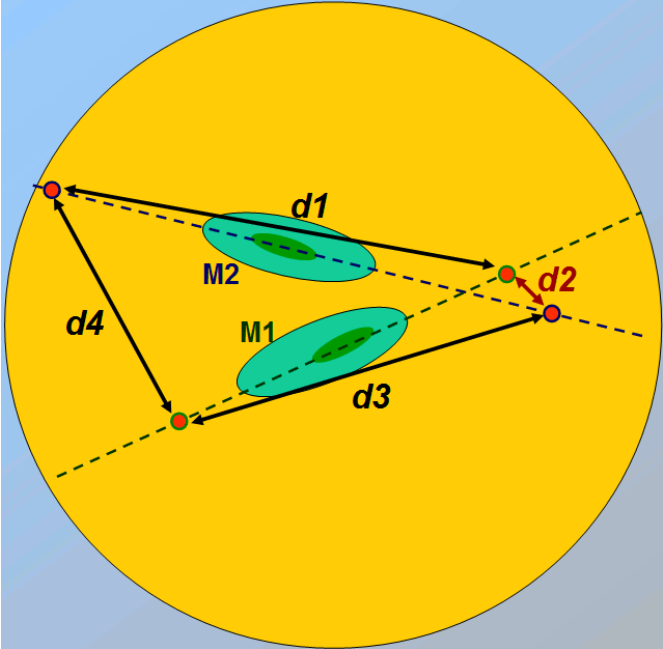
\includegraphics[width=0.5\textwidth]{./Plots/04_MrkAnalyse/Disp.png}
    \caption{Rekonstruktion des Parameters \texttt{Disp}. Dank der stereoskopischen Beobachtung, kann entschieden werden, welche Herkunftsrichtung für den Schauer am wahrscheinlichsten ist.\cite{DispRekonstruktion}}
    \label{Disp}
\end{figure}

Nur eine der beiden möglichen Quellpositionen des einen Teleskops ist kompatibel mit einer der rekonstruierten Quellpositionen des anderen Teleskops. 
Die bevorzugte Position der Quelle ist die, die näher am Schnittpunkt der beiden Hauptachsen liegt und bestimmt \texttt{Disp} für beide Teleskope eindeutig.
Letztendlich wird der gewichtete Mittelwert der beiden wahrscheinlichsten rekonstruierten Quellpositionen genommen.
Ereignisse mit einer zu großen Differenz der beiden rekonstruierten Quellpositionen zueinander werden verworfen.



\section{Berechnung der Lichtkurve}
\label{sec:Lichtkurve}
Der Gammafluss, d.h. die Rate der Gammateilchen $\frac{dN}{dt}$ pro Einheitsfläche ist Ausgangsgröße für die Lichtkurve:

\begin{equation}
 \Phi=\frac{d^2 N}{dS dt} 
\end{equation}
\begin{centering}
  \small{mit $N$: Anzahl der Teilchen, $S$: Fläche und $t$: Zeit.}
 \end{centering}
 
Dafür wird die Anzahl der detektierten Gammas, die effektive Observationszeit und die effektive Fläche des Detektors benötigt.
Nach der Energie differenziert ist diese Größe der differentielle Fluss pro Energie:

\begin{equation}
 \frac{d\Phi}{dE}=\frac{d^3N}{dSdtdE},
\end{equation}

bzw. der integrale Fluss:
\begin{equation}
 \Phi_{E>500GeV}=\int_{\SI{500}{GeV}}^{\infty}\frac{d\Phi}{dE}dE.
\end{equation}


Die zeitliche Entwicklung des integralen Flusses wird nun Lichtkurve genannt.
% Das Binning muss dabei so gewählt werden, dass die Statistik in jedem Bin groß genug ist.
% , tageweise oder minutenweise... Je nachdem, ob gerade irgendwas spannendes passiert (Flares oder so).

\subsection{Anzahl der Signalgammas}
Um die Anzahl der Gammateilchen aus der Quelle zu bestimmen, wird ein $\theta^2$-Histogramm benutzt.
Dies ist ein Histogramm der quadrierten Entfernungen zwischen der rekonstruierten Quellposition und der nominalen Quellposition.
Gammas aus der Quelle haben ein kleineres $\theta$ während der Background eine annähernd isotrope Verteilung liefert. 

\begin{figure}
    \centering
    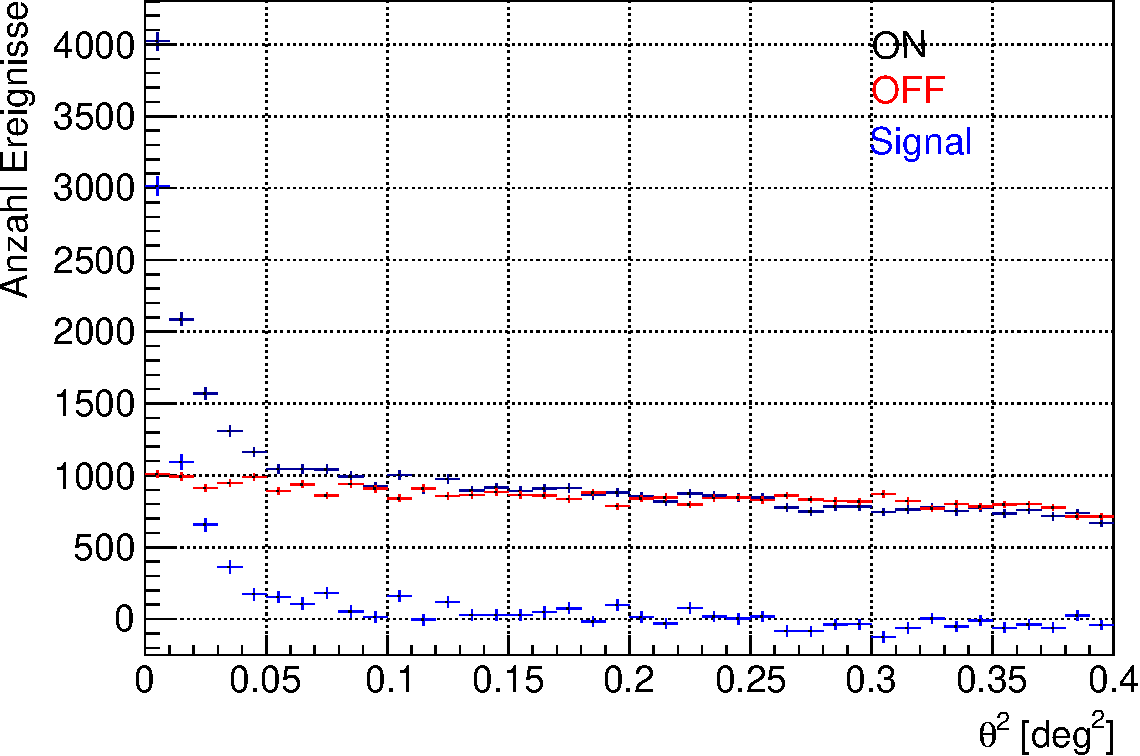
\includegraphics[width=0.8\textwidth]{./Plots/04_MrkAnalyse/Datenset2/Crab_Theta2.pdf}
    \caption{$\theta^2$-Verteilung von Crab-Datendes aus dem Datenset 2. Es ist zu sehen, dass die On- (Signal-) und die Off-(Background-) Daten für $\theta^2 > 0,1$ sehr gut aufeinander liegen.}
    \label{Disp}
\end{figure}
% BILDBILDBILD (abelardos talk in zeuthen, der auf der flute seite verlinkt ist)

Um die Anzahl der realen Signal-Ereignisse zu ermitteln, müssen von den Ereignissen aus der Quellrichtung noch die Background Ereignisse abgezogen werden und ein Schnitt in $\theta^2$ angewendet werden.

Dank der ``Wobble-Beobachtung`` ist eine simultane Datennahme von Signal- und Hintergrund möglich, d.h. das Teleskop ist nicht direkt auf die Quelle ausgerichtet, sondern die Quellposition ist $0.4°$ vom Kamerazentrum entfernt.
Wegen der Alt-Azimutalen Montierung rotiert die Quelle um das Zentrum in der Kamera und es ist möglich einen Punkt gegenüber der Quelle als Off-Position zu benutzen.
%Vorteil dieser Methode ist, dass es keine separate Off-Datennahme geben muss.
Es muss gewährleistet werden, dass die Off-Positionen symmetrisch verteilt sind, um Kamerainhomogenitäten entgegenzuwirken.
Allerdings tauchen bei dieser Methode die Quellgammas auch in der Off-$\theta^2$-Verteilung auf, haben aber ein großes $\theta^2$.
Eine Off-Position, die zu nahe an der Quelle ist, ist nicht zu empfehlen.

\subsection{Effektive Beobachtungszeit}
Die effektive Beobachtungszeit berücksichtigt die Totzeit in der Datennahme.
Nach dem Aufnehmen eines Ereignisses ist die Elektronik mit der Verarbeitung der Daten beschäftigt und neue Ereignisse können nicht detektiert werden.
Die Totzeit ist abhängig vom Chip und beträgt bei den aktuellen DRS4-Chips $\approx 26\mu$s.\todo{Quelle}

\subsection{Effektive Fläche}
Als effektive Fläche wird die Fläche am Boden bezeichnet, die orthogonal zur Herkunftsrichtung der Schauerteilchen ist.
Die Größe dieser effektiven Fläche ist abhängig von der Energie und dem Zenitwinkel des Schauers.
In \textit{MARS} wird diese Größe mit Hilfe von MCs folgendermaßen berechnet:

\begin{equation}
 A_{eff}(E)=\frac{N_{\gamma, final}}{N_{\gamma, simulated}}A_{MC, total}
\end{equation}

Dafür wird eine bestimmte Anzahl an Gammas ($N_{\gamma, simulated}$) auf einer uniformen Fläche $A_{MC,total}$ simuliert. 
Die Größe $N_{\gamma, final}$ ist die Anzahl der Gammas, die alle Analyseschnitte überlebt hat.


\section{Entfaltung des Energiespektrums}
\label{sec:Unfolding}
Bei der Messung mit IACTs handelt es sich um eine indirekte Messung.
Die Energie des Schauer-auslösenden Teilchens ist nicht direkt messbar.
Die Bildparameter und damit auch die geschätzte Energie $E_{est}$ haben eine begrenzte Auflösung und erfordern die Methode der Entfaltung.

Die Probleme, die bei der Messung auftreten, sind:

\begin{itemize}
 \item Begrenzte Akzeptanz: Nicht alle Schauer, die Teilchen auslösen, können vom Teleskop detektiert werden.
 \item Indirekte Messung: Da eine direkte Messung nicht möglich ist, wird anhand von gemessenen Parametern, wie z.B. der Größe des Schauers in der Kamera, mit Hilfe eines RF die Energie geschätzt.
       Die Vorraussetzung dafür ist, dass diese real gemessenen Parameter stark mit der Energie korrelliert sind.
 \item Begrenzte Auflösung: Es ist nur möglich mit begrenzter Genauigkeit aus den Bildparametern die Energie zu rekonstruieren, d.h. es existiert eine Migration von Ereignissen.
       Wird die geschätzte Energie gegen die reale Energie aufgetragen, erhält man eine verschmierte Diagonale (siehe Abb.\ref{EnergyEst_EnergyTrue})
\end{itemize}

\begin{figure}
    \centering
    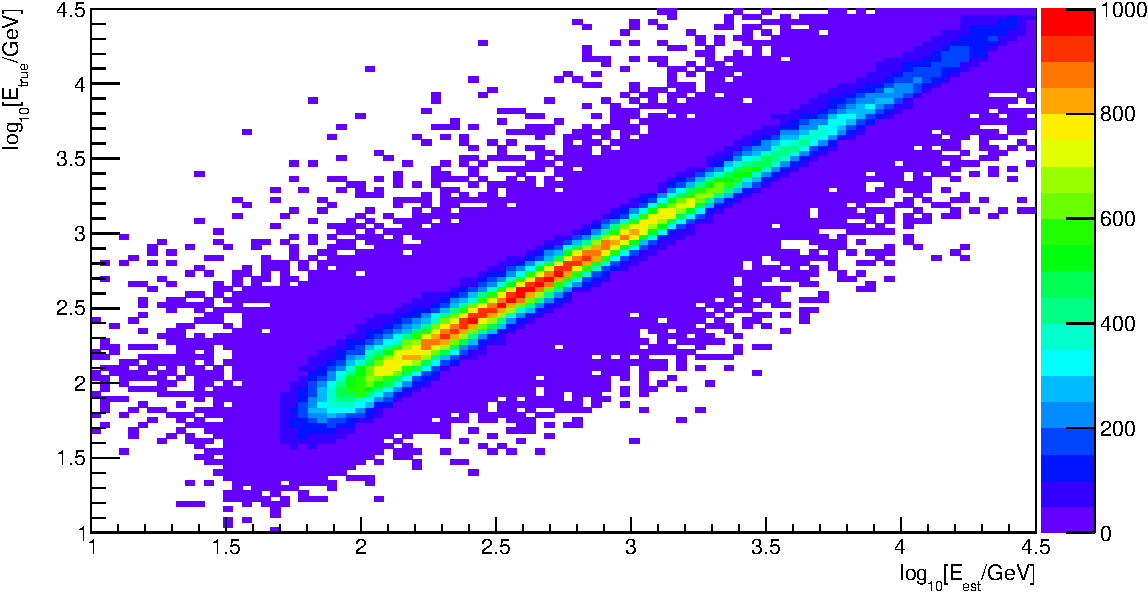
\includegraphics[width=0.8\textwidth]{./Plots/04_MrkAnalyse/EnergyEst_EnergyTrue.pdf}
    \caption{Geschätzte Energie gegen wahre Energie. Es ist erkennbar, dass keine perfekte Energierekonstruktion existiert.}
    \label{EnergyEst_EnergyTrue}
\end{figure}

Durch die Methode der Entfaltung können diese Probleme berücksichtigt werden. 
Das Problem lässt sich mit einer Fredholmschen Integralgleichung darstellen:

\begin{equation}
 g(y)= \int_c^d M(x,y) f(x) dx + b(y)
\end{equation}
\begin{centering}
  \tiny{mit g(y): gemessene Verteilung, f(x): gesuchte Verteilung, M(x,y): Migrationsmatrix bestimmt auf MCs, b(y): Background-Verteilung}
 \end{centering}

Diese Gleichung lässt sich auch diskretisiert darstellen:

\begin{equation}
 g_i=\sum_j M_{ij}f_j+b_i,
\end{equation}

wobei $M_{ij}$ die Migrationsmatrix ist und damit die Wahrscheinlichkeit beschreibt, dass ein Ereignis in bin j in bin i gezählt wird.

Das Ziel der Entfaltung ist die wahre Verteilung $f$ zu finden.
Die Kovarianzmatrix der gesuchten Verteilung ergibt sich dann mit der Kovarianzmatrix der gemessenen Verteilung zu:

\begin{equation}
 \mathbf{V[\vec{f}]}=\mathbf{M}^{-1}\mathbf{V}[\vec{g}]\mathbf{(M}^{-1})^T
\end{equation}

Da die Invertierung der Migrationsmatrix oft zu oszillierenden Lösungen führt, versucht man die Methode der kleinsten Quadrate.

\begin{equation}
 \chi_0^2=(\vec{g}-\mathbf{M}\vec{f})^T \mathbf{V}^{-1}[\vec{g}](\vec{g}-\mathbf{M}\vec{f}).
\end{equation}

Dies gilt nur für Gaußverteilte Daten, also nicht für Bins mit kleinen Ereigniszahlen.
Für diese muss nun die Poisson-Statistik benutzt werden und der Log-Likelihood-Ausdruck minimiert werden:

\begin{equation}
 L_0(a)=\sum_i (g_i(a)-g_{i,m}\cdot \ln g_i(a)).
\end{equation}

Außerdem ist es nötig, eine Regularisierung einzuführen, um die kleinen Ausdrücke in der Migrationsmatrix, die während der Entfaltung verstärkt werden, zu unterdrücken.
Durch Einführung eines Regularisierungsterms werden Anforderungen an die Lösung gestellt, bei zu starker Regularisierung aber auch ein Bias eingeführt.

Im Allgemeinen wird Regularisierung durch Addition eines Regularisierungsterms gemacht, sodass:

\begin{equation}
 \chi^2=\chi_0^2 +\frac{\tau}{2} Reg(f).
\end{equation}

Verschiedene Arten der Regularisierung können in der Analyse gewählt werden.
Es ist auch möglich, eine Vorwärtsfaltung durchzuführen, wobei ein bestimmtes Modell als Annahme gewählt wird und freie Parameter dieses Modells bestimmt werden.
Zum Testen ist dies eine gute Alternative, allerdings keine richtige Entfaltung, da das Ergebnis modellabhängig bleibt und physikalische Phänomene verborgen bleiben.

\section{Mrk 421-Analyse}
\label{Mrk421_Analyse}
In diesem Abschnitt wird die Analyse der Daten beschrieben, wobei für jede der vier Datenepochen sowohl Lichtkurve als auch Spektrum gezeigt werden.
Dabei wird die Analyse des Datensatz 2 der Daten exemplarisch für die Stereo-Analyse erklärt (\autoref{subsec:Datenset_2}), während die anderen Zeitabschnitte des Jahres mit stereoskopischer Beobachtung (\autoref{subsec:Datenset_1} und \autoref{subsec:Datenset_4}) analog ausgewertet werden.
Auf die Mono-Datenanalyse wird in \autoref{subsec:Datenset_3} eingegangen.
Zusammenfassend wird noch eine Lichtkurve aller Daten gezeigt.


\subsection{Überblick über die Daten}
Die Daten, die für diese Analyse zur Verfügung standen, sind Daten der Quelle Mrk 421, die 2012 genommen wurden.
Die Daten gliedern sich folgendermaßen:

\begin{itemize}
 \item Datenset 1: 2012-02-25 - 2012-02-29
 \item Datenset 2: 2012-03-18 - 2012-04-27
 \item Datenset 3: 2012-05-23 - 2012-06-19 (Mono)
 \item Datenset 4: 2012-12-11 - 2012-12-23
\end{itemize}

Datenset 1 und Datenset 2 sind beides Stereobeobachtungen.
Die beiden Datensets unterscheiden sich in ihrer PSF (Point Spread Function), weswegen zwei verschiedene MC-Sets in der Analyse verwendet werden.
Die PSF beschreibt die Abbildungsqualität der Spiegel, bzw. wie gut sie ausgerichtet sind.
Je größer die PSF ist, umso schlechter sind die Abbildungseigenschaften und um so verschmierter ist die Reflexion einer Punktquelle.

Beim 3. Datenset handelt es sich um Mono-Daten. 
Aufgrund der defekten MAGIC-I-Kamera und der geplanten Upgrade-Pause, wurde nur MAGIC-II betrieben.

Im 4. Datenset war das Upgrade abgeschlossen, die alte MAGIC-I-Kamera durch eine neue Kamera ersetzt und es wurden wieder Stereo-Beobachtungen durchgeführt.
Aufgrund der Hardware-Veränderungen und einer anderen PSF wurden wieder neue MCs produziert.

Die Analyse des ersten Datensets befindet sich in \autoref{subsec:Datenset_1} und die des zweiten Datensets in \autoref{subsec:Datenset_2}.
Danach erfolgt die dritte Analyseperiode mit Stereobeobachtungen in \autoref{subsec:Datenset_4}.
Die Mono-Analyse wird zuletzt in \autoref{subsec:Datenset_3} beschrieben.


\subsection{Datenset 2}
\label{subsec:Datenset_2}
Anhand der genommenen Mrk 421-Daten, zehn Tage zwischen dem 18.3.2012 (MJD: 56004.1) und dem 27.4.2012 (MJD: 56042.0), wird nun die Stereo-Analyse erklärt.

Diese Daten wurden in einem Zenitwinkelbereich zwischen 12° und 30° genommen (siehe Abb.\ref{Datenset2_fZD}).

\begin{figure}
    \centering
    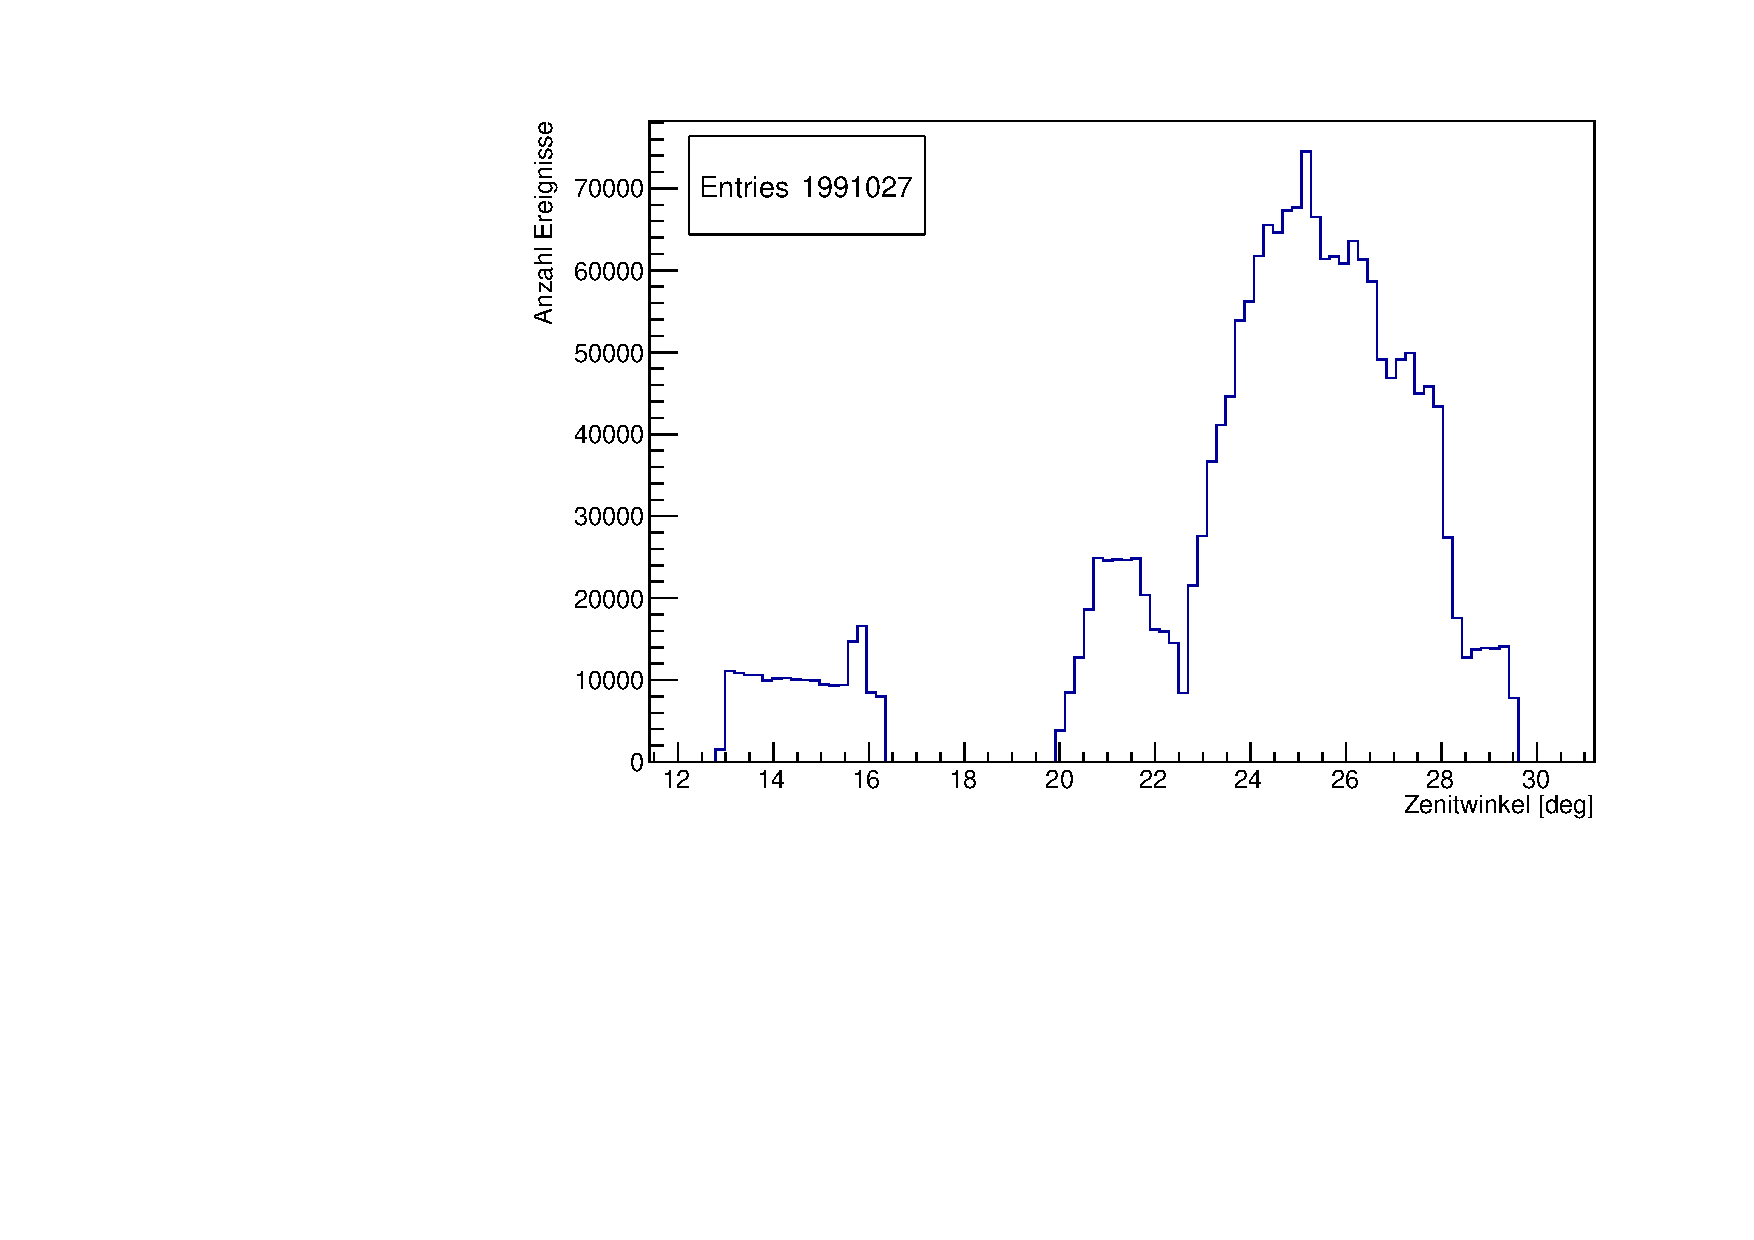
\includegraphics[width=0.7\textwidth]{./Plots/04_MrkAnalyse/Datenset2/Datenset2_Mrk421_MPointingPos_fZd.pdf}
    \caption{Zenitverteilung der genommenen Mrk 421-Daten zwischen dem 18.3.2012 und dem 27.4.2012.}
    \label{Datenset2_fZD}
\end{figure}


Da dieser Datensatz die meisten Daten beinhaltet, wird die Analyse exemplarisch hiermit durchgeführt.

Als Off-Daten dienen Daten anderer Quellen, welche in der gleichen Zeitspanne wie die zu analysierende liegen.
Dadurch wird gewährleistet, dass das Teleskop die gleichen Eigenschaften, wie z.B. PSF, hat wie bei der Datennahme der zu analysierenden Quelle. 

Mit Hilfe von Crab-Daten werden die Einstellungen für die Lichtkurvenbestimmung gesucht, da Crab als Standardkerze dient und einen bekannten stabilen Fluss hat. 


\subsubsection{Daten-Auswahl und Qualitätchecks}
Zunächst werden die auf \textit{Superstar}-Level prozessierten Daten einem Datencheck unterzogen, um die Daten herauszufiltern, die bei guten Bedingungen genommen wurden.
Gute Bedingungen sind durch dunkle Nächte, wenig Störlicht durch z.B. Autoscheinwerfer und keine Hardware- oder Softwareprobleme gekennzeichnet.

Um dunkle Bedingungen zu gewährleisten wurde zunächst ein Cut im Direct Current (DC) (MI < 500nA, M II < 800nA) durchgeführt.
Danach wurden mit Hilfe des \textit{MARS} Macros \textit{Quate} alle Daten mit einem Zenitwinkel < 35° ausgewählt, Runs mit einer Länge unter 10s und Runs mit einer Abweichung des Pointings von 15arcmin verworfen.
Außerdem wurden die Mittelwerte der Rate, der Parameter \texttt{Number of Islands}, \texttt{Concentration}, \texttt{Width} und \texttt{Length} gebildet und ebenfalls Ausreißer aussortiert um eine gute Qualität der Daten zu gewährleisten.

Diese Kriterien für den Datencheck wurden für die Mrk 421-Daten, die Crab-Daten und die Off-Daten angewendet.

In der Tabelle \ref{tab:Datenset2-Mrk421} ist aufgelistet, an welchen Tagen Mrk 421-Daten nach dem Datencheck für die Analyse zur Verfügung stehen.


\begin{table}[!h]
\centering
\caption{Diese Tabelle zeigt, für welche Tage Mrk 421-Daten nach dem Datencheck zur Analyse zur Verfügung stehen.}
\label{tab:Datenset2-Mrk421}
\begin{tabular}{ll}
  \toprule
  Monat & Tage\\
  \midrule
  \midrule
März & 18., 22., 28.\\
April & 11., 13., 15., 19., 21., 23., 25. \\
  \bottomrule
\end{tabular}
\end{table}

Tabelle \ref{tab:Datenset2} zeigt wieviele Minuten Daten, Background-Daten und Crab-Daten den Datencheck überstanden haben. 
Auf eine tageweise Auflistung der Background- und Crab-Daten wird verzichtet.

\begin{table}[!h]
\centering
\caption{Diese Tabelle zeigt eine Übersicht über die Menge an Mrk 421-, Crab- und Background-Daten nach dem Datencheck.}
\label{tab:Datenset2}
\begin{tabular}{lc}
  \toprule
  Quelle & Observationszeit\\
  \midrule
  \midrule
  Mrk 421 & 272min\\
  \midrule
  Crab & 161min\\
  \midrule
  0FGLJ0631 & 77min \\
  1ES1011 & 492min \\
  1ES1426 & 424min \\
  PG1553 & 971min \\
  PKS1222 & 247min \\
  SegueJ & 3252min \\
  \bottomrule
\end{tabular}
\end{table}

Für diesen Teil der Analyse werden die in Dortmund produzierten Standard-MC-Daten im Zenitbereich 5°-35° genommen, in denen die alte MAGIC-I Kamera simuliert wurde.
Die PSF für MAGIC-I beträgt hierbei 10.5mm und die Mirror Fraction 0.58, während diese Werte für MAGIC-II 10.2mm für die PSF und 0.70 für die Mirror Fraction sind.

Es ist zu beachten, dass für alle Daten (Mrk 421/Crab/Off) und die MCs das gleiche Cleaning benutzt wird, da zu dieser Zeit zwei verschiedene Cleaning-Schwellen im Next-Neighbor-Cleaning gebräuchlich waren.
Die Core und Neighbor-Schwelle beträgt in diesen Daten 6, bzw. 3.


\subsubsection{\textit{Coach} und \textit{Melibea}}
Für das Training des RF für die GH-Separation und die \texttt{Disp}-Bestimmung sowie das Erstellen der Look-Up-Tables zur Energierekonstruktik ist es wichtig, dass in jedem Zenitbin genug Background- und MC-Daten vorhanden sind.
Es wird ein Zenitbereich von 10-35° ausgewählt.
Wie in Abb.\ref{Datenset2_Zenitverteilung_Off} und Abb.\ref{Datenset2_Zenitverteilung_MC} zu sehen ist, ist diese Voraussetzung erfüllt.

\begin{figure}
    \centering
    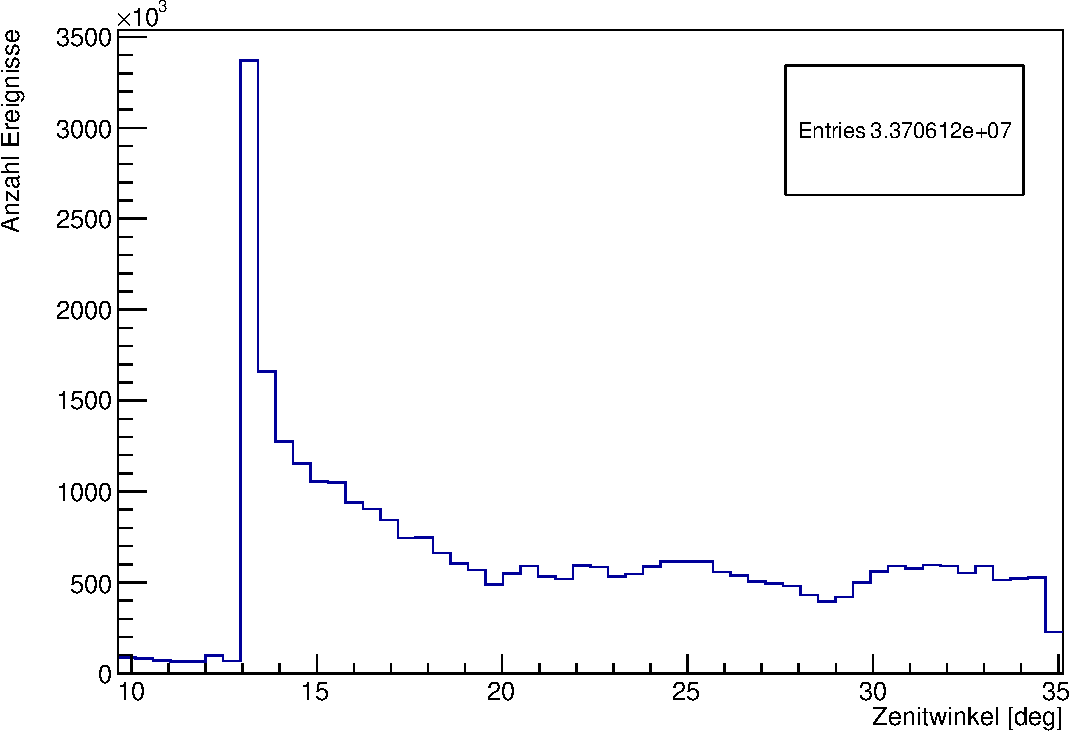
\includegraphics[width=0.7\textwidth]{./Plots/04_MrkAnalyse/Datenset2/Datenset2_Background_MPointingPos1_fZd.pdf}
    \caption{Zenitverteilung der Off-Daten zwischen dem 18.3.2012 und dem 27.4.2012. Leere Bins sind nicht enthalten.}
    \label{Datenset2_Zenitverteilung_Off}
\end{figure}

\begin{figure}
    \centering
    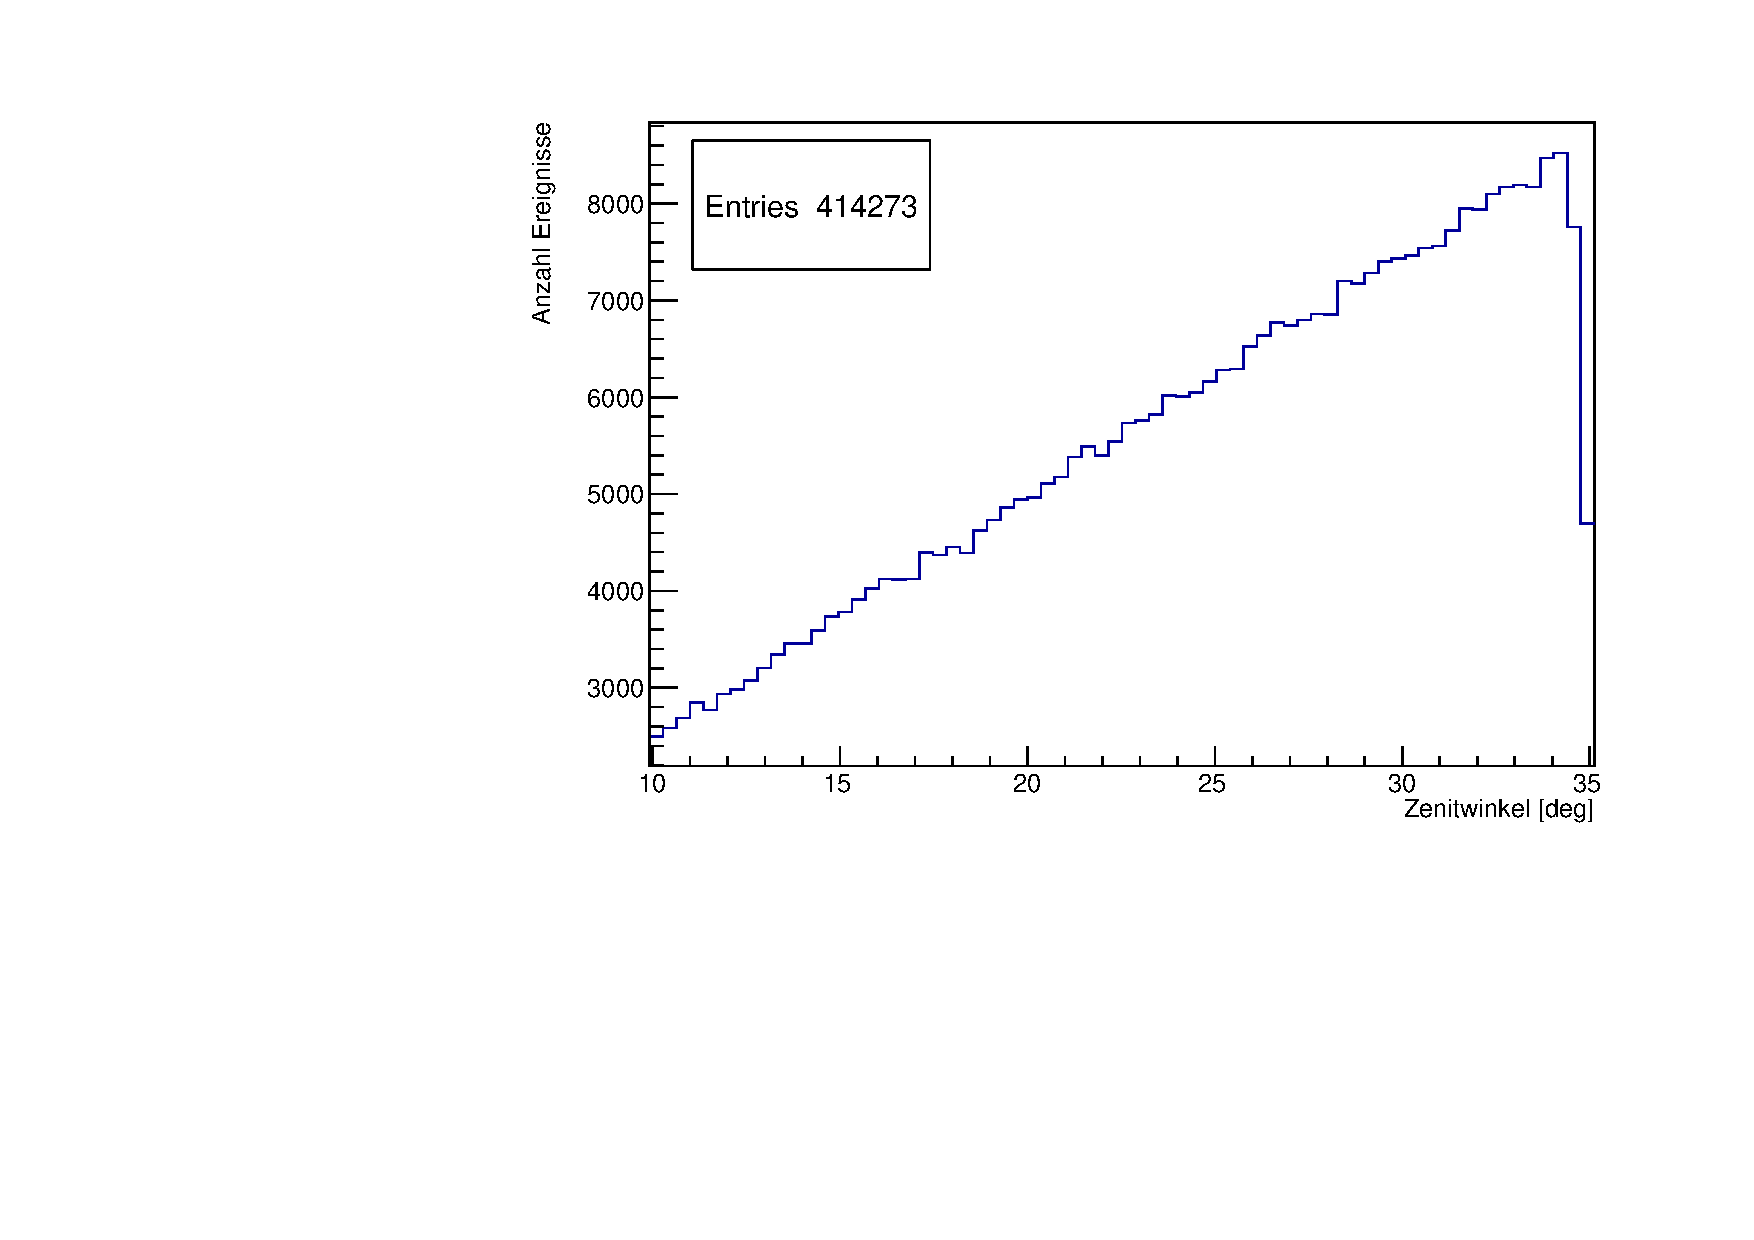
\includegraphics[width=0.7\textwidth]{./Plots/04_MrkAnalyse/Datenset2/Datenset2_MC_MPointingPos1_fZd.pdf}
    \caption{Zenitverteilung des Trainingssets der MC.}
    \label{Datenset2_Zenitverteilung_MC}
\end{figure}

Der MC-Datensatz wurde in zwei Teile geteilt.
Der eine Teil, das Trainings-Set, wird zusammen mit den Off-Daten zum Trainieren des RF für die GH-Separtion und für Disp benutzt, sowie zum Aufstellen der Look-Up-Tables für die Energie.
Der andere Teil wird später zur Entfaltung benutzt.

Sobald das Training der RFs und das Erstellen der Look-Up-Tables in \textit{Coach} beendet ist, werden in \textit{Melibea} die Daten nach Gamma- und Hadron-Ereignis klassifiziert und jedem Ereignis eine geschätzte Energie und ein \texttt{Disp}-Wert zugeordnet.
Das gleiche geschieht auch mit den Crab-Daten und dem anderen Teil der MCs, dem Test-Set.


\subsubsection{Lichtkurve von Crab}
Wie in \autoref{sec:Lichtkurve} beschrieben, wird nun sowohl für die Crab-Daten als auch für die Mrk 421 Daten eine Lichtkurve erstellt.
Da der Fluss von Crab stabil und bekannt ist, werden mit Hilfe der Crab-Daten die passenden Parameter (Hadroneffizienz und $\theta$-Quadrat-Effizienz) für die Lichtkurven-Bestimmung in diesem Zeitraum für Mrk 421 ausgewählt.

Wie in Abb.\ref{Datenset2_Flute_Plots_Crab} zu sehen, ist es möglich mit Flute neben der Lichtkurve (vgl. Abb.\ref{Datenset2_LC_Crab}) auch noch einen $\theta$ Quadrat Plot (vgl. Abb.\ref{Datenset2_theta^2_Crab}), sowie die spektrale Energie-Verteilung (vgl. Abb.\ref{Datenset2_SED_Crab}) zu berechnen.

\begin{figure}
  %-----------------------------Figure 1--------------------------------------------------------%
  \begin{subfigure}{0.45\linewidth}
  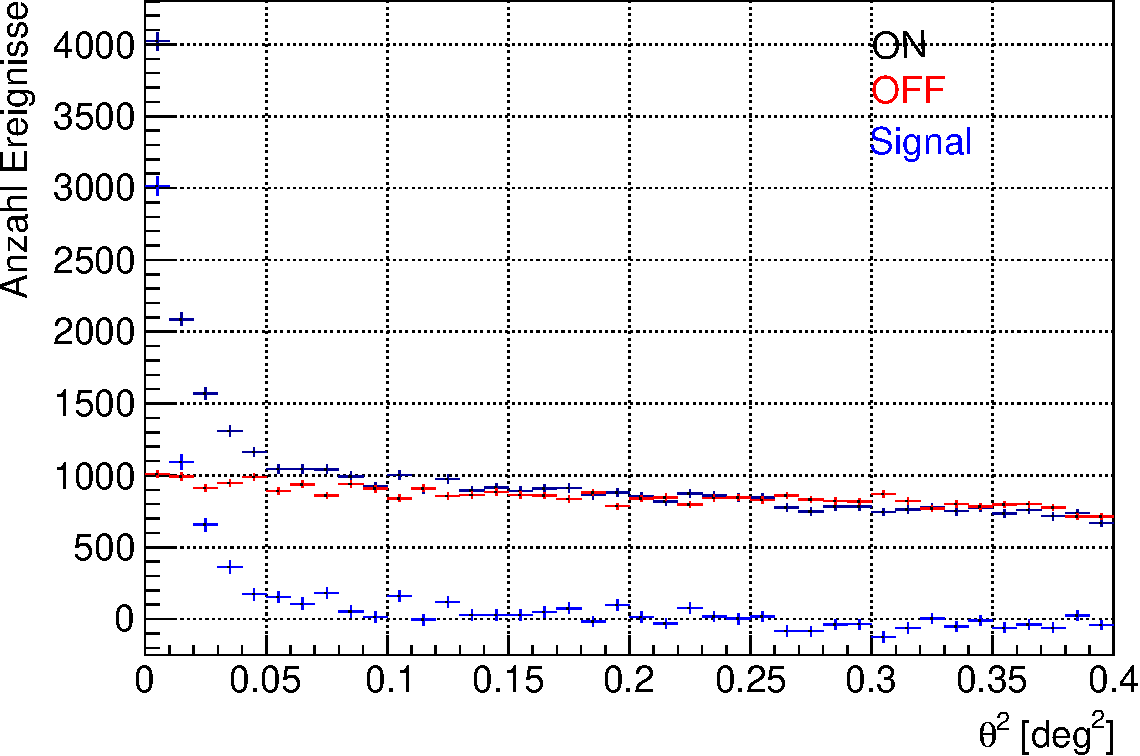
\includegraphics[width=\textwidth]{./Plots/04_MrkAnalyse/Datenset2/Crab_Theta2.pdf}
  \caption{$\theta^2$-Plot für Crab für alle Wobble-Positionen}
  %für den Energiebereich zwischen 5.5 GeV und 55.43TeV
  \label{Datenset2_theta^2_Crab}
  \end{subfigure}
  \hfill
  %-----------------------------Figure 2--------------------------------------------------------%
  \begin{subfigure}{0.45\linewidth}
  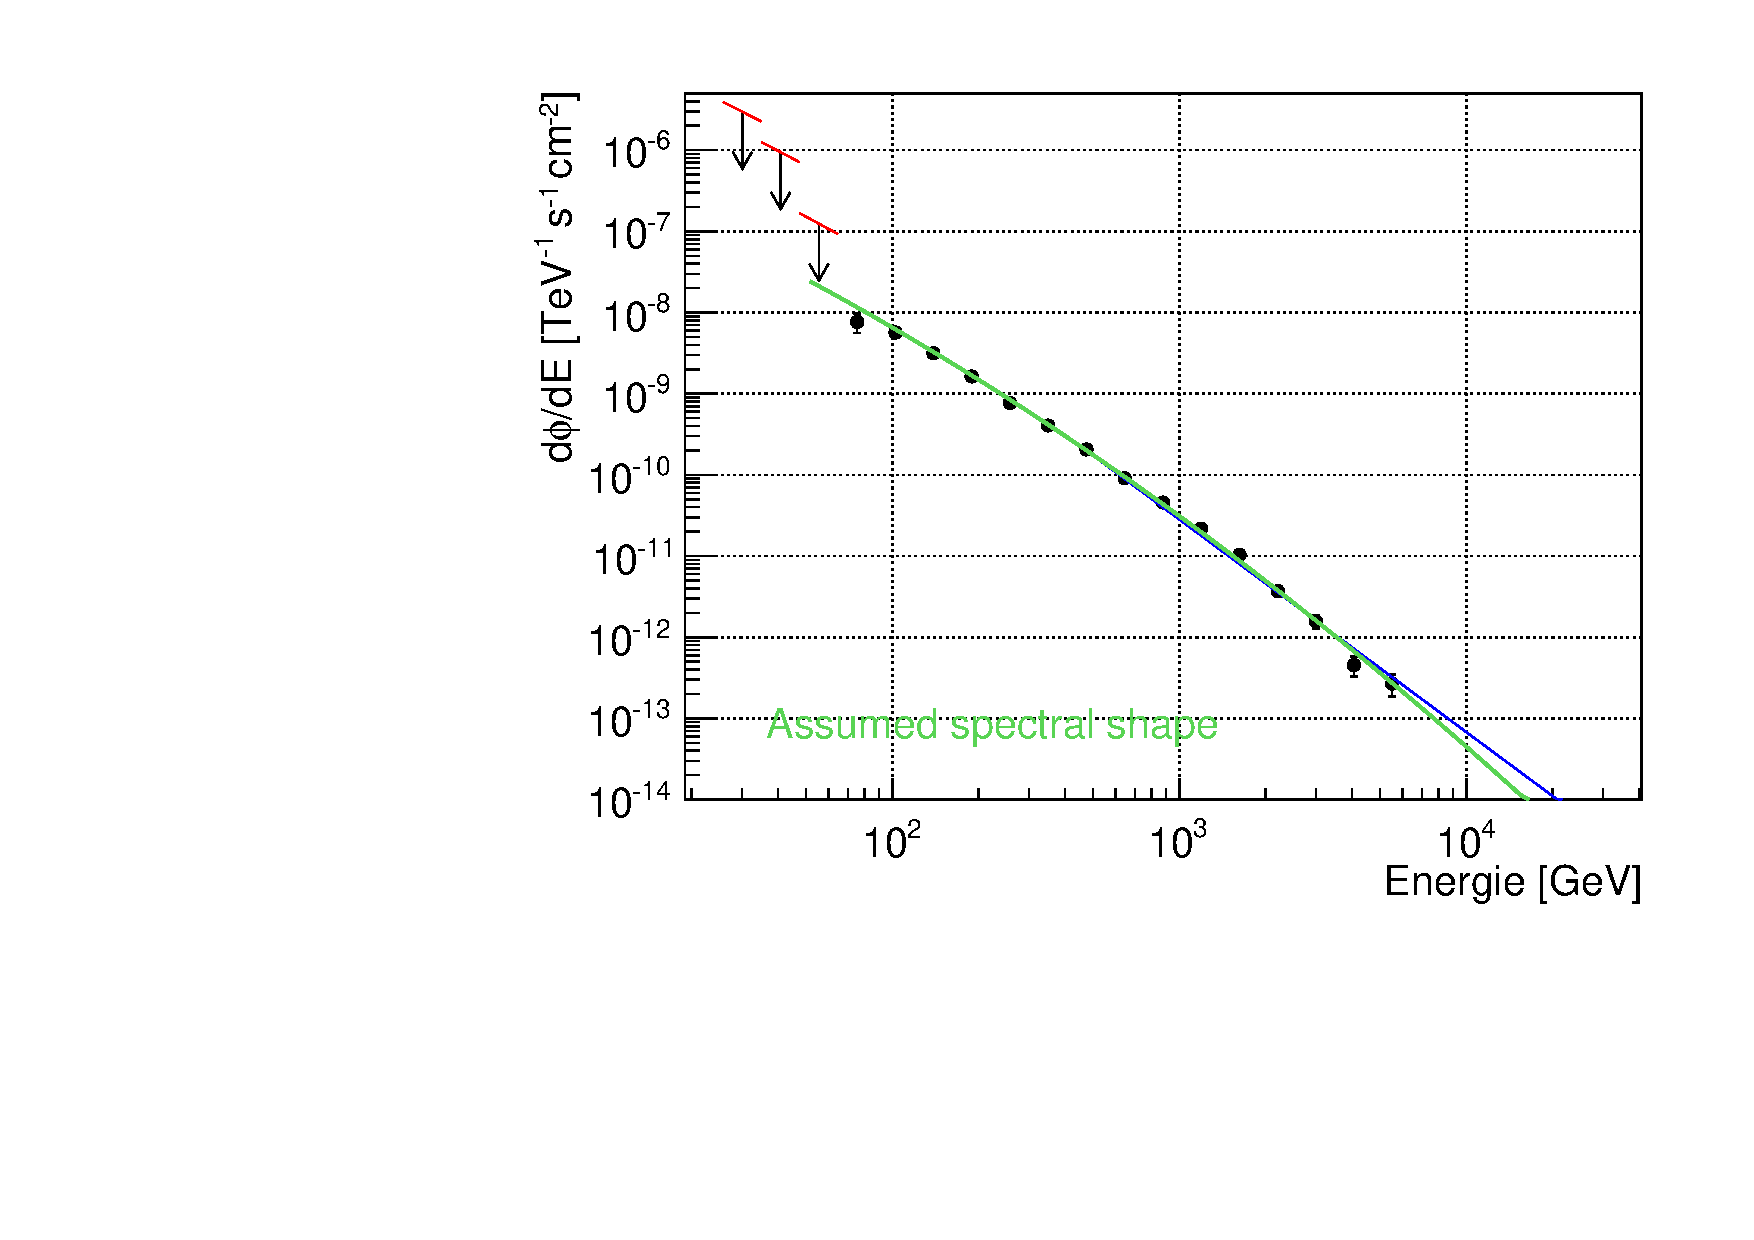
\includegraphics[width=\textwidth]{./Plots/04_MrkAnalyse/Datenset2/Crab_dFdE.pdf}
  \caption{Differentielles Energiespektrum}
  \label{Datenset2_SpectralShape_Crab}
  \end{subfigure}
  \hfill
  %-----------------------------Figure 3--------------------------------------------------------%
  \begin{subfigure}{0.45\linewidth}
  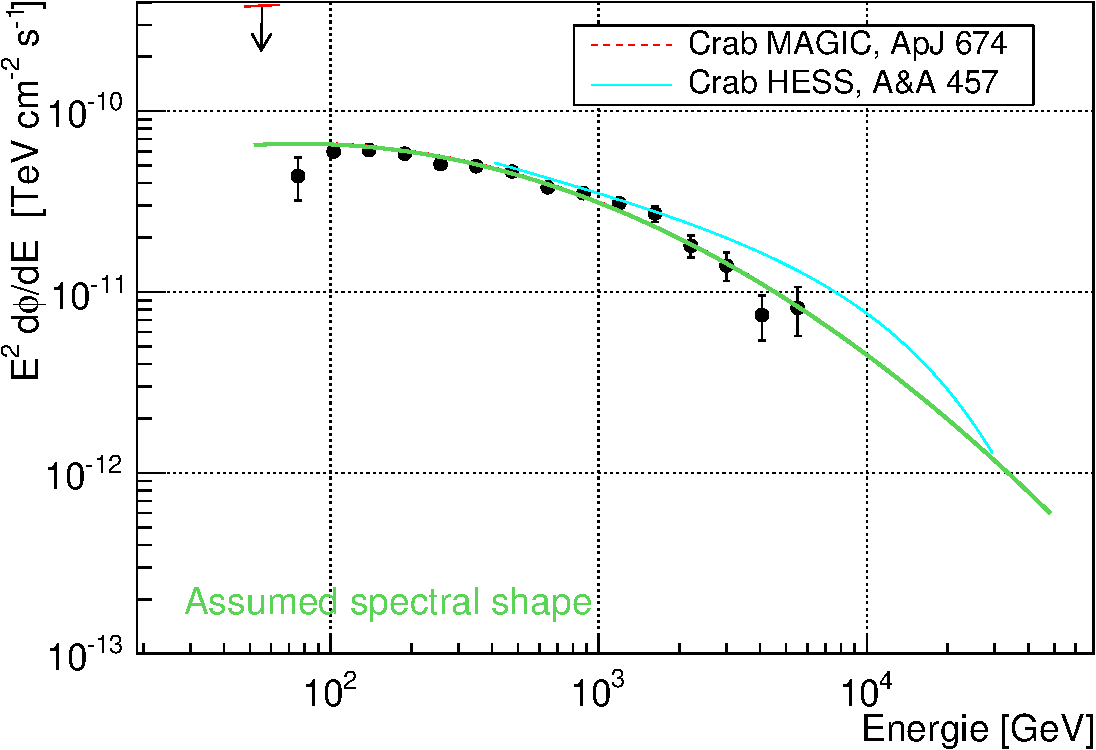
\includegraphics[width=\textwidth]{./Plots/04_MrkAnalyse/Datenset2/Crab_SED.pdf}
  \caption{Spektrale Energieverteilung}
  \label{Datenset2_SED_Crab}
  \end{subfigure}
  \hfill
  %-----------------------------Figure 4--------------------------------------------------------%
  \begin{subfigure}{0.45\linewidth}
  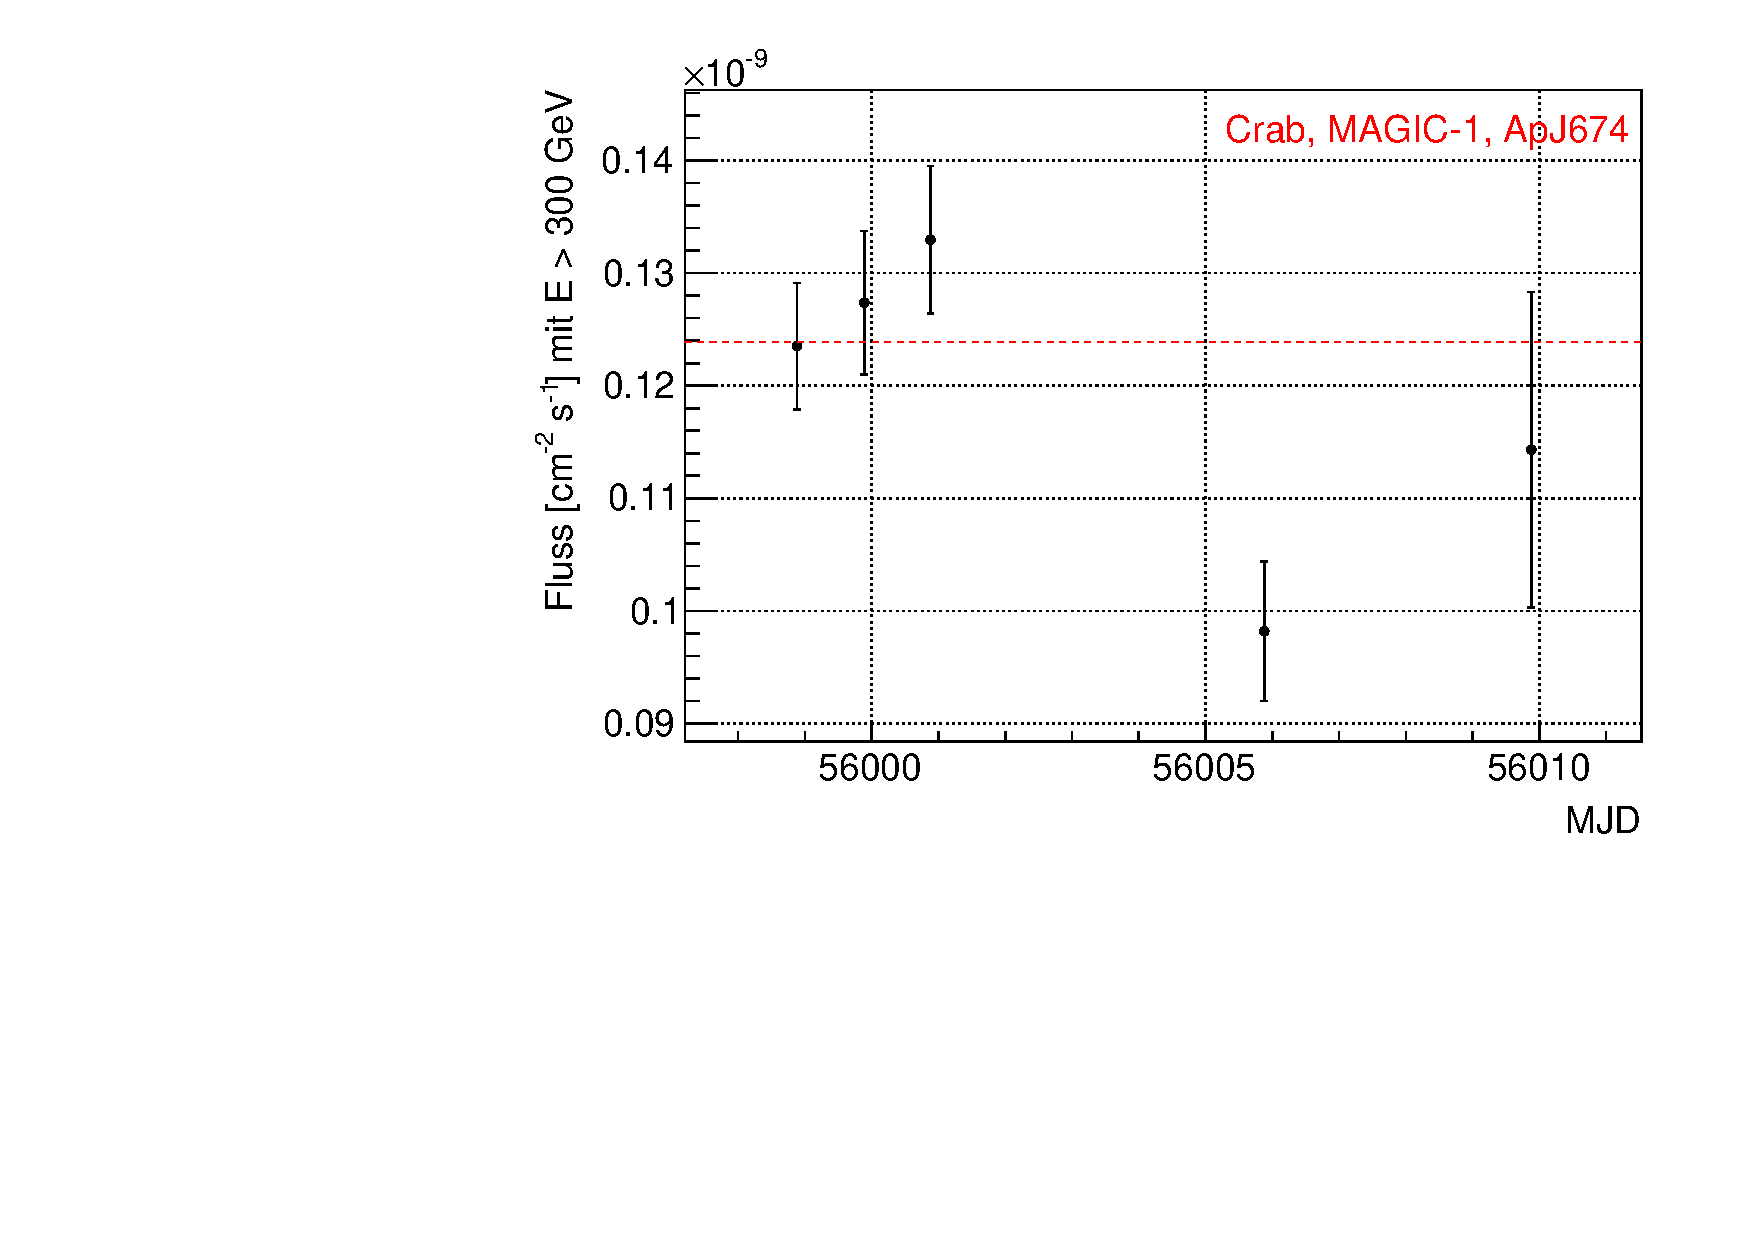
\includegraphics[width=\textwidth]{./Plots/04_MrkAnalyse/Datenset2/Crab_LC.pdf}
  \caption{Lichtkurve von Crab mit mittlerem Fluss von Crab}
  \label{Datenset2_LC_Crab}
  \end{subfigure}
  \hfill
  %----------------------------------------------------------------------------------------------%
\caption{\textit{Flute}-Plots für Crab}
\label{Datenset2_Flute_Plots_Crab}
\end{figure}

In Abb.\ref{Datenset2_theta^2_Crab} ist der $\theta^2$-Plot für Crab zu sehen, für kleine $\theta$ ist die Anzahl der Signal-Ereignisse wie zu erwarten sehr hoch.
In Abb.\ref{Datenset2_SpectralShape_Crab} ist das differentielle Energiespektrum zu sehen.
Abb.\ref{Datenset2_SED_Crab} zeigt die spektrale Energieverteilung.
Wie in Abb.\ref{Datenset2_SpectralShape_Crab} und in Abb.\ref{Datenset2_SED_Crab} zu sehen ist, passt das angenommene Spektrum gut zu den Daten, bzw. zum bekannten Crab-Spektrum.
Angenommen wurde folgendes Spektrum:

\begin{equation}
\frac{dN}{dE}=\left(\frac{x}{\SI{300}{GeV}}\right)^{-2.31-0.26\cdot \text{log10}(x/300.)}\si{TeV\,cm^{-2}\,s^{-1}}
 %pow(x/300.,-2.31-0.26*log10(x/300.))
\end{equation}

Die Lichtkurve in Abb.\ref{Datenset2_LC_Crab} zeigt, dass der Crab-Fluss in diesem Zeitraum um den mittleren Crab-Fluss schwankt.
Die Parameter, die zum Erstellen der Lichtkurve in \textit{Flute} verwendet wurden, erweisen sich also als vernünftig.

\subsubsection{Lichtkurve von Mrk 421}
Es wird nun mit den gleichen Effizienz-Einstellungen wie für Crab eine Lichtkurve für Mrk 421 angefertigt.

\begin{figure}
    \centering
    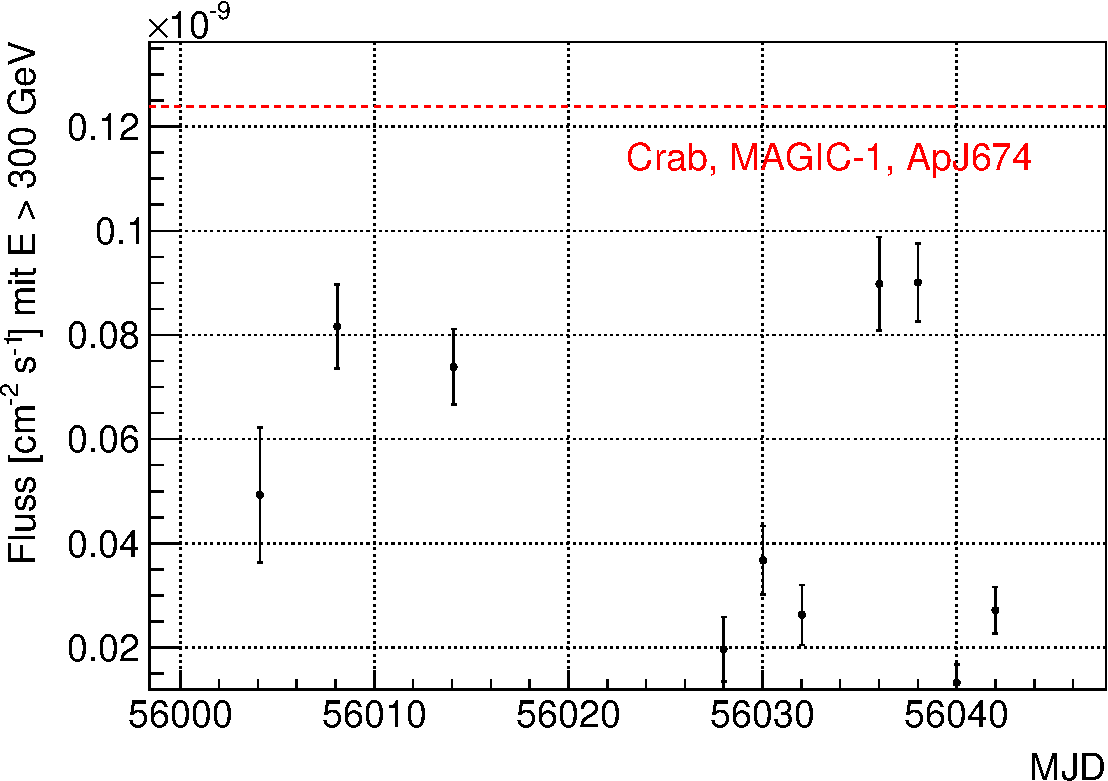
\includegraphics[width=0.8\textwidth]{./Plots/04_MrkAnalyse/Datenset2/LC_Mrk421.pdf}
    \caption{Lichtkurve von Mrk 421.}
    \label{Datenset2_LC_Mrk421}
\end{figure}

Abb.\ref{Datenset2_LC_Mrk421} zeigt, dass der Fluss von Mrk 421 im Vergleich zu Crab wesentlich niedriger ist.
Er schwankt etwa um den halben Crab-Fluss.
Auch die spektrale Energieverteilung sieht anders aus (vgl. Abb.\ref{Datenset2_SED_Mrk421}), da ein anderes Spektrum angenommen wurde:

\begin{equation}
\frac{dN}{dE}=\left(\frac{x}{\SI{300}{GeV}}\right)^{-2.75}\si{TeV\,cm^{-2}\,s^{-1}}
\end{equation}


\begin{figure}
    \centering
    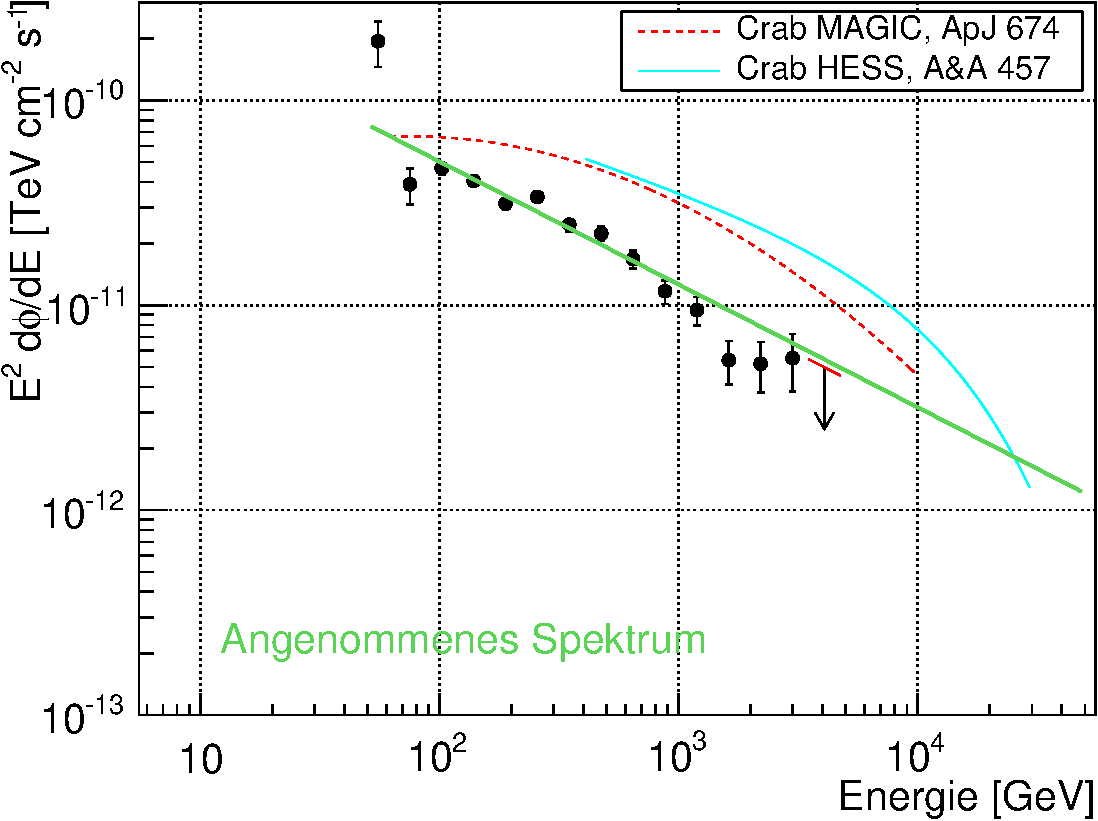
\includegraphics[width=0.8\textwidth]{./Plots/04_MrkAnalyse/Datenset2/SED_Mrk421.pdf}
    \caption{Spektrale Energieverteilung von Mrk 421.}
    \label{Datenset2_SED_Mrk421}
\end{figure}


\subsubsection{Spektrum von Crab}
Mit Hilfe von CombUnfold wird nun das Spektrum von Crab entfaltet.
Abb.\ref{Datenset2_CombunFold_Crab} zeigt das entfaltete Spektrum von Crab mit Literaturwert.

\begin{figure}
    \centering
    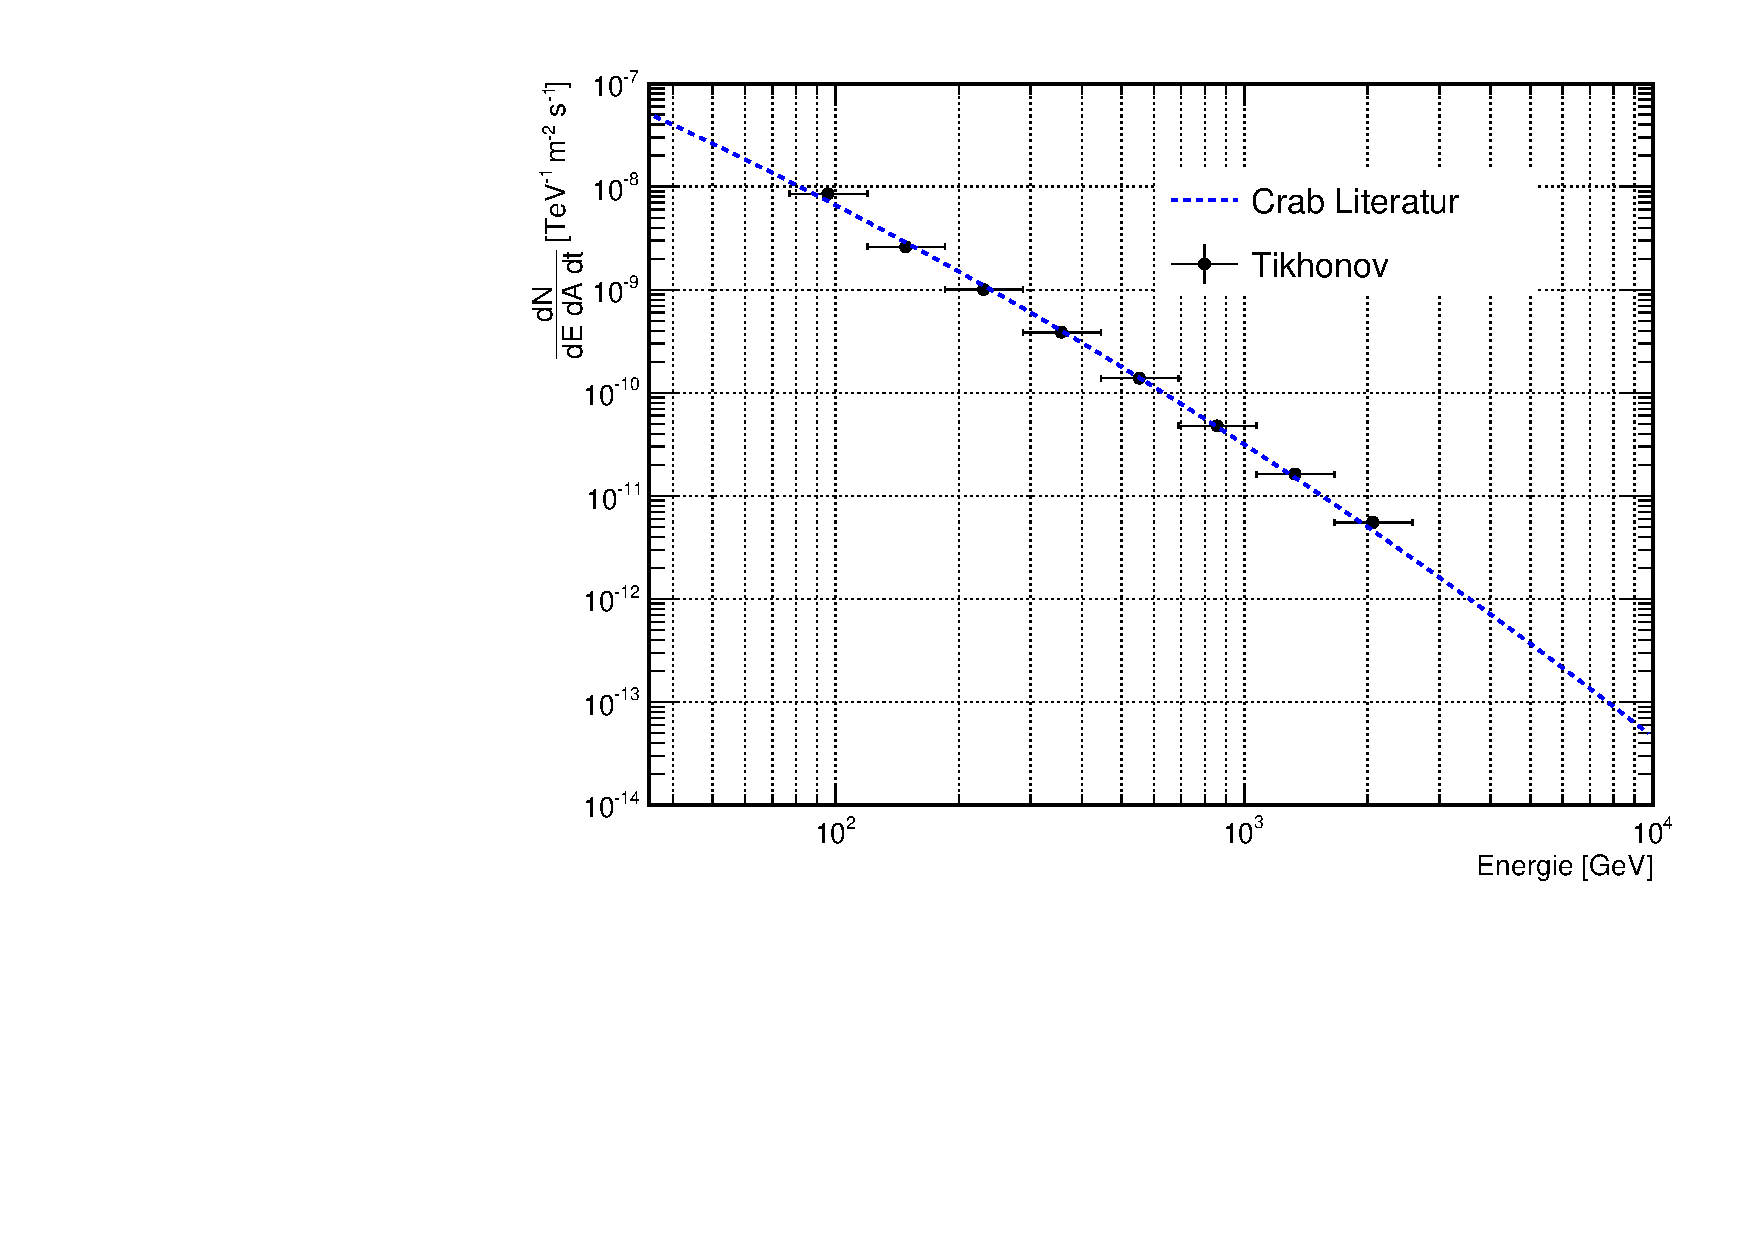
\includegraphics[width=0.8\textwidth]{./Plots/04_MrkAnalyse/Datenset2/Crab_mit_Literatur.pdf}
    \caption{Entfaltetes Crab-Spektrum mit Literaturwerten.}
    \label{Datenset2_CombunFold_Crab}
\end{figure}

Es zeigt sich, dass die entfalteten Datenpunkte mit Tikhonov-Regularisierung sehr gut zum Literaturwert passen.

\subsubsection{Spektrum von Mrk 421}
Abb.\ref{Datenset2_CombunFold_Mrk421} zeigt das entfaltet Spektrum von Mrk 421 mit fünf verschiedenen Regularisierungsmethoden.
Wie man sieht, zeigen die entfalteten Datenpunkte keine großen Abweichung voneinander. 
Lediglich bei kleinen Energien unterscheiden sich die Ergebnisse etwas.

\begin{figure}
    \centering
    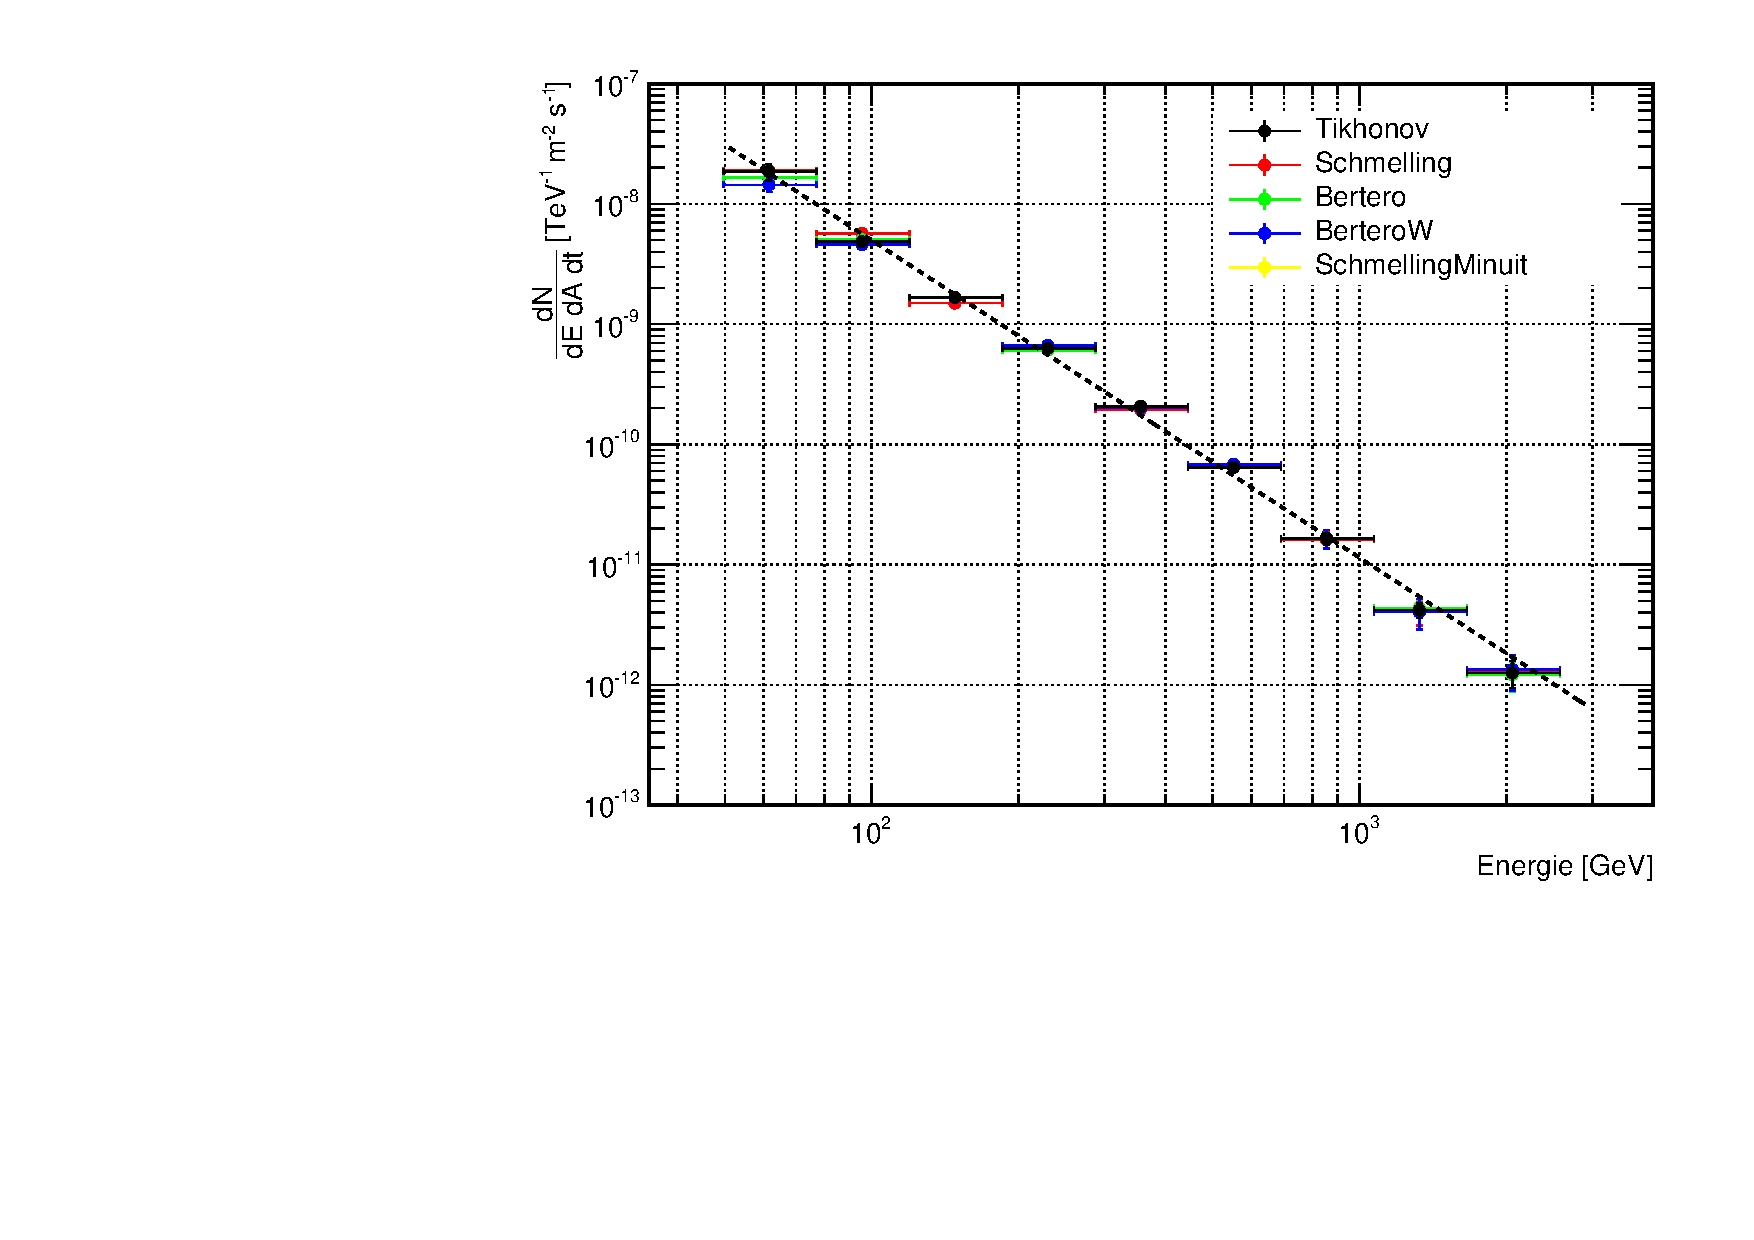
\includegraphics[width=0.8\textwidth]{./Plots/04_MrkAnalyse/Datenset2/Spektrum_Mrk421.pdf}
    \caption{Entfaltetes Mrk 421-Spektrum mit allen möglichen Regularisierungssorten}
    \label{Datenset2_CombunFold_Mrk421}
\end{figure}

Es wurde der Fit, der in der Entfaltung mit Tikhonov-Regularisierung erstellt wurde zusätzlich dargestellt, da diese Regularisierungsmethode in den meisten Fällen die besten Ergebnisse lieferte.
Folgende Funktion wurde angenommen:

\begin{equation}
 \frac{dN}{dE\,dA\,dt}=f_0\left( \frac{E}{r} \right)^\alpha.
\end{equation}

Der Fit lieferte das Ergebnis:

\begin{equation}
 \frac{dN}{dE\,dA\,dt}=2,74 \cdot 10^{-10}\left( \frac{E}{\SI{0,3}{TeV}} \right)^{-2.64} \si{TeV^{-1}\,s^{-1}\,cm^{-2}}.
\end{equation}


\FloatBarrier

\subsection{Datenset 1}
\label{subsec:Datenset_1}
Der folgende Teil handelt von der kurzen Analyse der Daten vom 25.2.2012 und 29.2.2012.
Da diese Daten eine andere PSF haben als die Daten aus Datenset 2, gibt es eigene MCs dafür und die Daten müssen getrennt von Datenset 2 analysiert werden.
Die Daten an diesen zwei Tagen haben ebenfalls einen Zenitbereich bis 35°.

\subsubsection{Datencheck}
Der Datencheck für diese Daten geschieht analog zum Datencheck des Datensets 2. 
Tabelle \ref{tab:Datenset1-Mrk421} zeigt an welchen Tagen Mrk 421-Daten den Datencheck überstanden haben und für die Analyse zur Verfügung stehen. 

\begin{table}[!h]
\centering
\caption{Diese Tabelle zeigt, für welche Tage Mrk 421-Daten nach dem Datencheck zur Analyse zur Verfügung stehen.}
\label{tab:Datenset1-Mrk421}
\begin{tabular}{ll}
  \toprule
  Monat & Tage\\
  \midrule
  \midrule
Februar & 25., 29.\\
  \bottomrule
\end{tabular}
\end{table}


Tabelle \ref{tab:Datenset1} zeigt wieviel Mrk 421-/Crab- und Off-Daten den Datencheck überstanden haben.


\begin{table}[!h]
\centering
\caption{Daten nach Datencheck}
\label{tab:Datenset1}
\begin{tabular}{lc}
  \toprule
  Quelle & Obersvationszeit\\
  \midrule
  \midrule
  Mrk 421 & 70min\\
  \midrule
  Crab & 20min\\
  \midrule
  0FGLJ0631 & 3min \\
  1ES1011 & 172min \\
  HB89 & 87min \\
  PG1553 & 115min \\
  PKS1222 & 106min \\
  SegueJ & 401min \\
  \bottomrule
  \bottomrule
\end{tabular}
\end{table}

\subsubsection{Lichtkurve}
Mit Hilfe von Crab-Daten wurden wieder die Einstellungen für die Lichtkurve von Mrk 421 bestimmt.
Die Lichtkurve von Crab beinhaltet nur 20min an Daten an einem Tag (vgl. Abb.\ref{Datenset1_LC_Crab}).

\begin{figure}
    \centering
    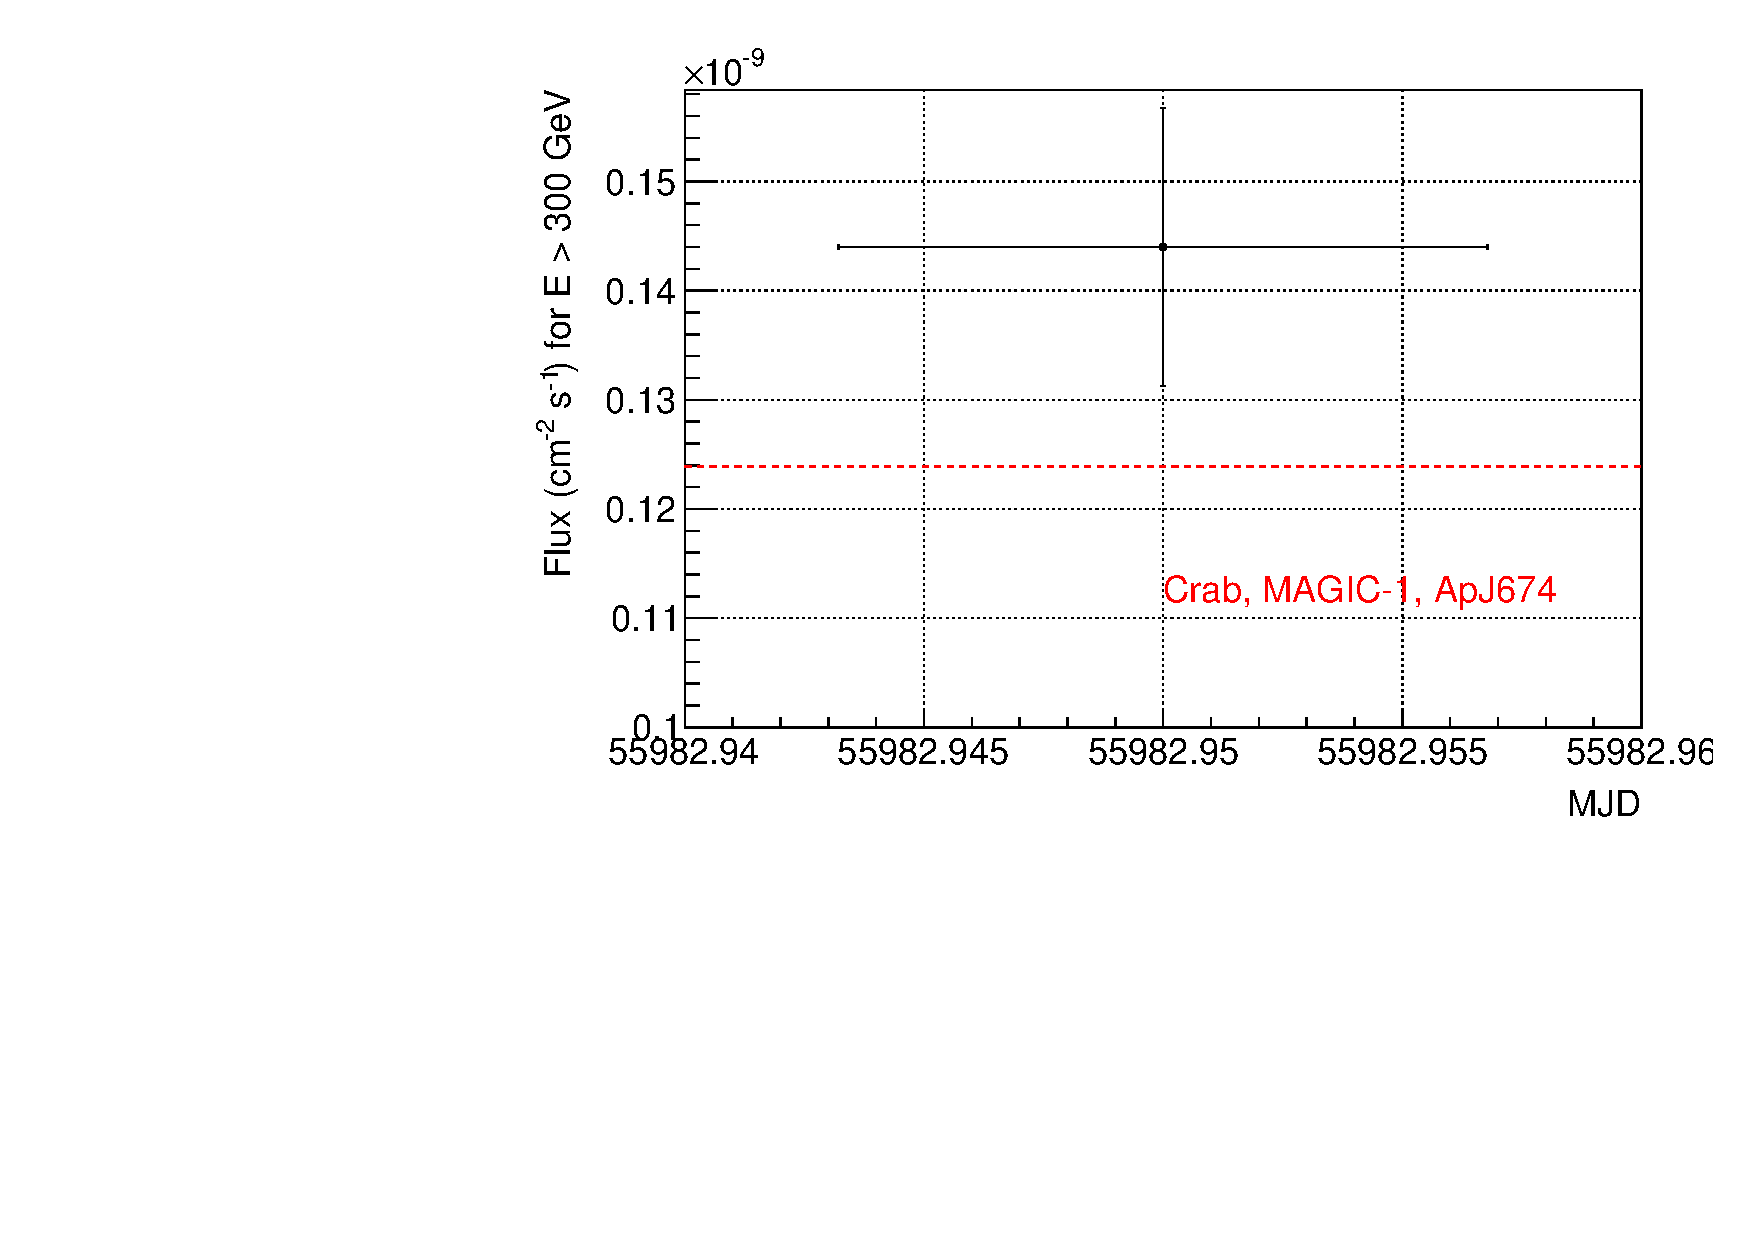
\includegraphics[width=0.8\textwidth]{./Plots/04_MrkAnalyse/Datenset1/Datenset1_LC_Crab.pdf}
    \caption{LC von Crab.}
    \label{Datenset1_LC_Crab}
\end{figure}

Die Lichtkurve von Mrk 421 befindet sich in Abb.\ref{Datenset1_LC_Mrk421}.

\begin{figure}
    \centering
    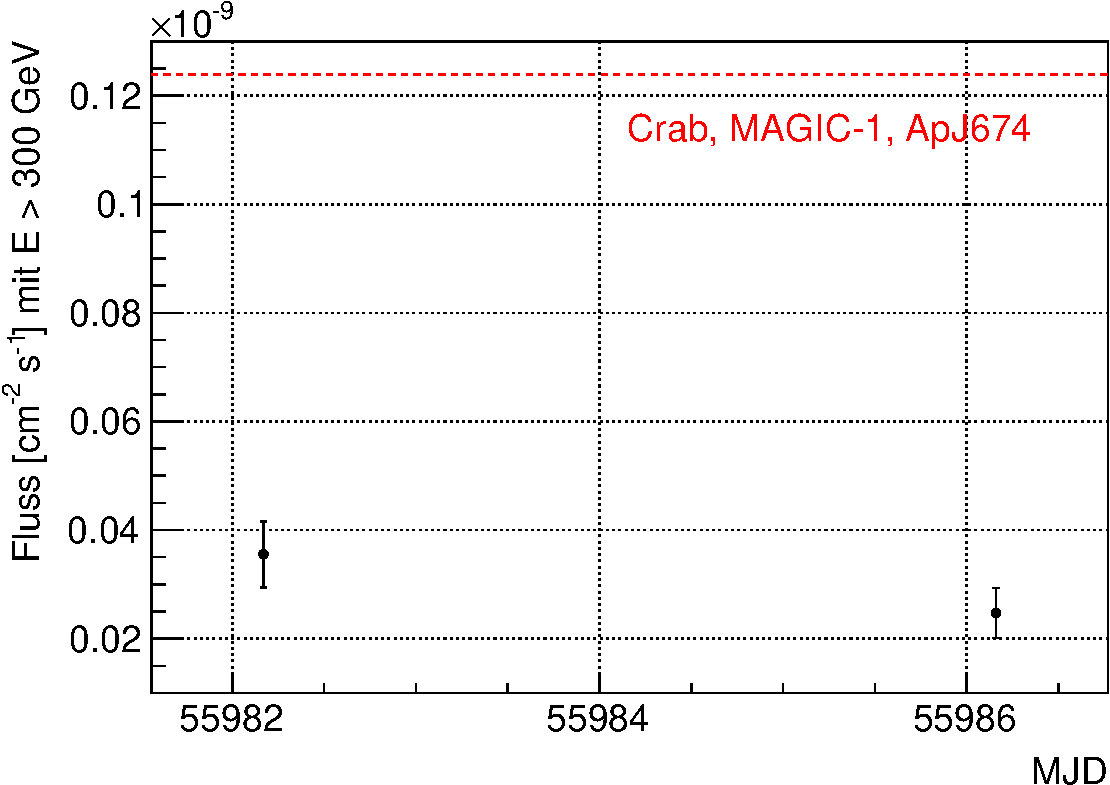
\includegraphics[width=0.8\textwidth]{./Plots/04_MrkAnalyse/Datenset1/Datenset1_LC_Mrk421.pdf}
    \caption{Lichtkurve von Mrk 421.}
    \label{Datenset1_LC_Mrk421}
\end{figure}

Es ist zu sehen, dass der Fluss an diesen beiden Tagen verglichen mit den ersten Tagen aus Datenset 2 sehr niedrig ist.



\FloatBarrier

\subsubsection{Spektrum}
Analog zu Datenset 2 wurde auch wieder ein Spektrum bestimmt.
Das Resultat befindet sich in Abb.\ref{Datenset1_Spektrum_Mrk421}

\begin{figure}
    \centering
    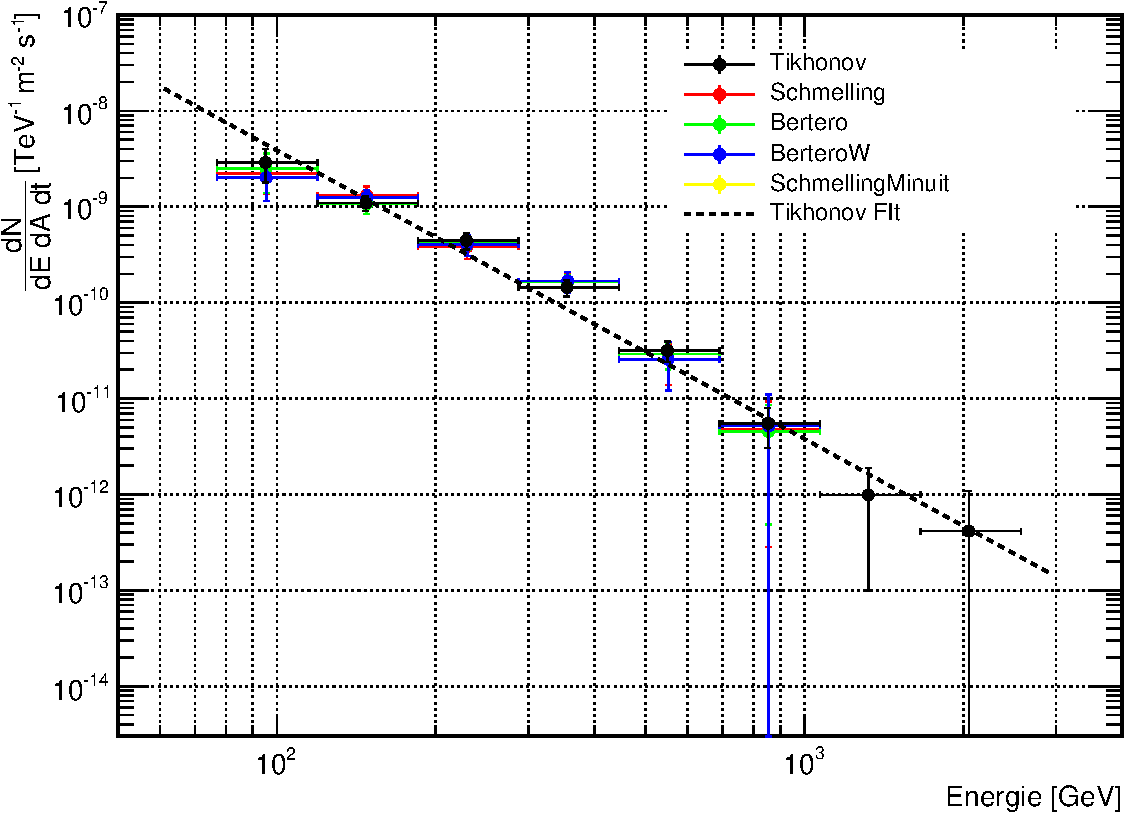
\includegraphics[width=0.8\textwidth]{./Plots/04_MrkAnalyse/Datenset1/Spektrum_Mrk421.pdf}
    \caption{Spektrum von Mrk 421.}
    \label{Datenset1_Spektrum_Mrk421}
\end{figure}

Es ist zu sehen, dass die Entfaltungen ohne Tikhonov-Regularisierung im hohen Energiebereich nicht mehr funktionieren.
Auch bei kleinen Energien unterscheiden sie sich etwas.
Aufgrund des großen Energiebereichs, in dem die Entfaltung mit Tikhonov-Regularisierung Ergebnisse liefert, wird wieder dieser Fit der Punkte eingezeichnet.
Der Fit lieferte folgendes Ergebnis:

\begin{equation}
 \frac{dF}{dE}=1,42 \cdot 10^{-11}\left( \frac{E}{0,3 \si{TeV}} \right)^{-3.01} \si{TeV^{-1}\,s^{-1}\,cm^{-2}}.
\end{equation}

Auf Grund der kurzen Observationszeit wurde keine Entfaltung der Crab-Daten vorgenommen.

\FloatBarrier

\subsection{Datenset 4}
\label{subsec:Datenset_4}
Dieses Datenset beinhaltet die ersten Daten, die von Mrk 421 nach dem Austausch der MAGIC-I-Kamera genommen wurden. 
Genauso wie Datenset 1 umfasst dieses Datenset nur wenige Tage. 
An drei Tagen wurde Mrk 421 im Stereo-Modus observiert. 

\subsubsection{Datencheck}
Der Datencheck für diese Daten geschieht analog zum Datencheck des Datensets 2. 
Tabelle \ref{tab:Datenset4} zeigt, welche Mrk 421-/Crab- und Off-Daten nach dem Datencheck übrig sind und Tabelle \ref{tab:Datenset4-Mrk421} an welchen Tage die Mrk 421-Daten genommen wurden.

\begin{table}[!h]
\centering
\caption{Diese Tabelle zeigt, für welche Tage Mrk 421-Daten nach dem Datencheck zur Analyse zur Verfügung stehen.}
\label{tab:Datenset4-Mrk421}
\begin{tabular}{ll}
  \toprule
  Monat & Tage\\
  \midrule
  \midrule
Dezember & 15., 19., 23.\\
  \bottomrule
\end{tabular}
\end{table}


\begin{table}[!h]
\centering
\caption{Daten nach Datencheck}
\label{tab:Datenset4}
\begin{tabular}{lc}
  \toprule
  Quelle & Observationszeit\\
  \midrule
  \midrule
  Mrk 421 & 74min\\
  \midrule
  Crab & 852min\\
  \midrule
  1ES0229 & 221min \\
  NGC1275 & 112min \\
  SegueA & 900min  \\
  \bottomrule
  \bottomrule
\end{tabular}
\end{table}

\subsubsection{Lichtkurve}
Die Lichtkurve von Crab befindet sich in Abb. \ref{Datenset4_LC_Crab}.
und die Lichtkurve von Mrk 421 in Abb.\ref{Datenset4_LC_Mrk421} 
Wie zu sehen ist, liegen auch hier die Flüsse niedrig.

\begin{figure}
    \centering
    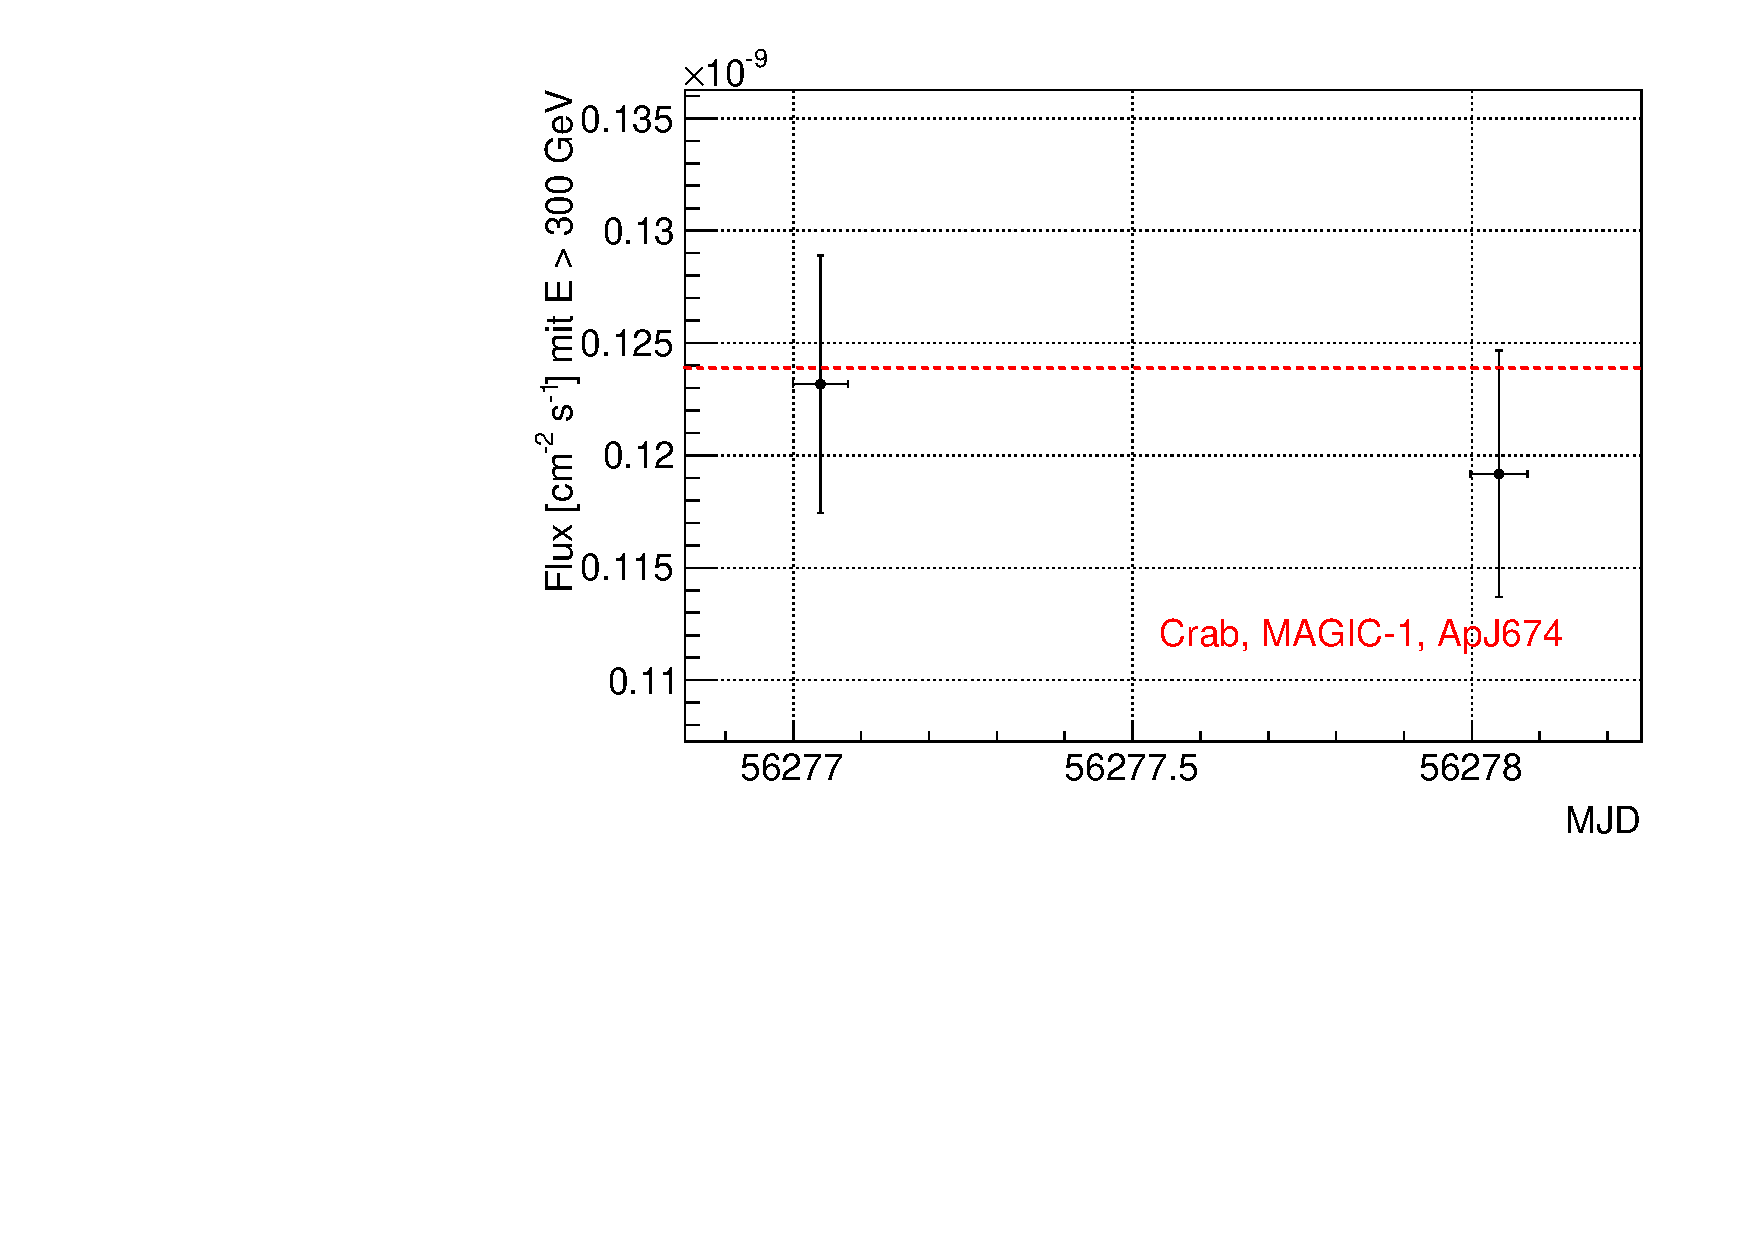
\includegraphics[width=0.8\textwidth]{./Plots/04_MrkAnalyse/Datenset4/Datenset4_LC_Crab.pdf}
    \caption{Lichtkurve Crab.}
    \label{Datenset4_LC_Crab}
\end{figure}

\begin{figure}
    \centering
    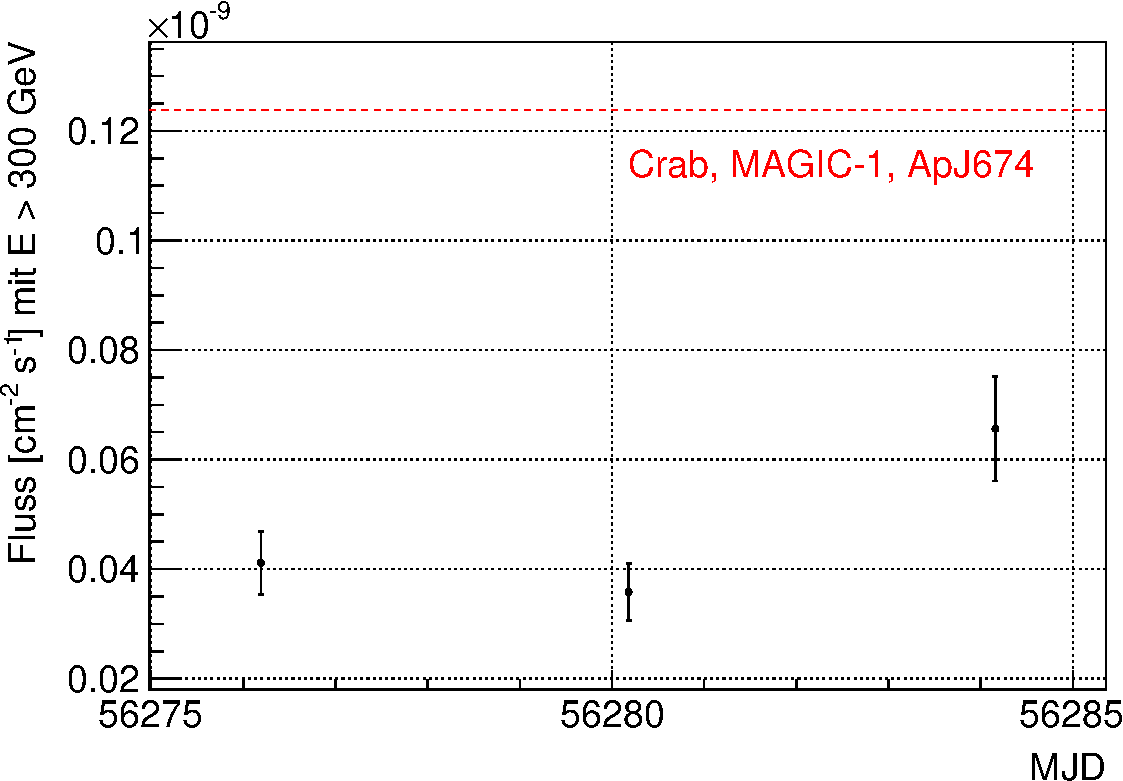
\includegraphics[width=0.8\textwidth]{./Plots/04_MrkAnalyse/Datenset4/Datenset4_LC_Mrk421.pdf}
    \caption{Lichtkurve Mrk 421.}
    \label{Datenset4_LC_Mrk421}
\end{figure}


\subsubsection{Spektrum}
Das entfaltete Spektrum von Mrk 421 befindet sich in Abb.\ref{Datenset4_Spektrum_Mrk421}.

\begin{figure}
    \centering
    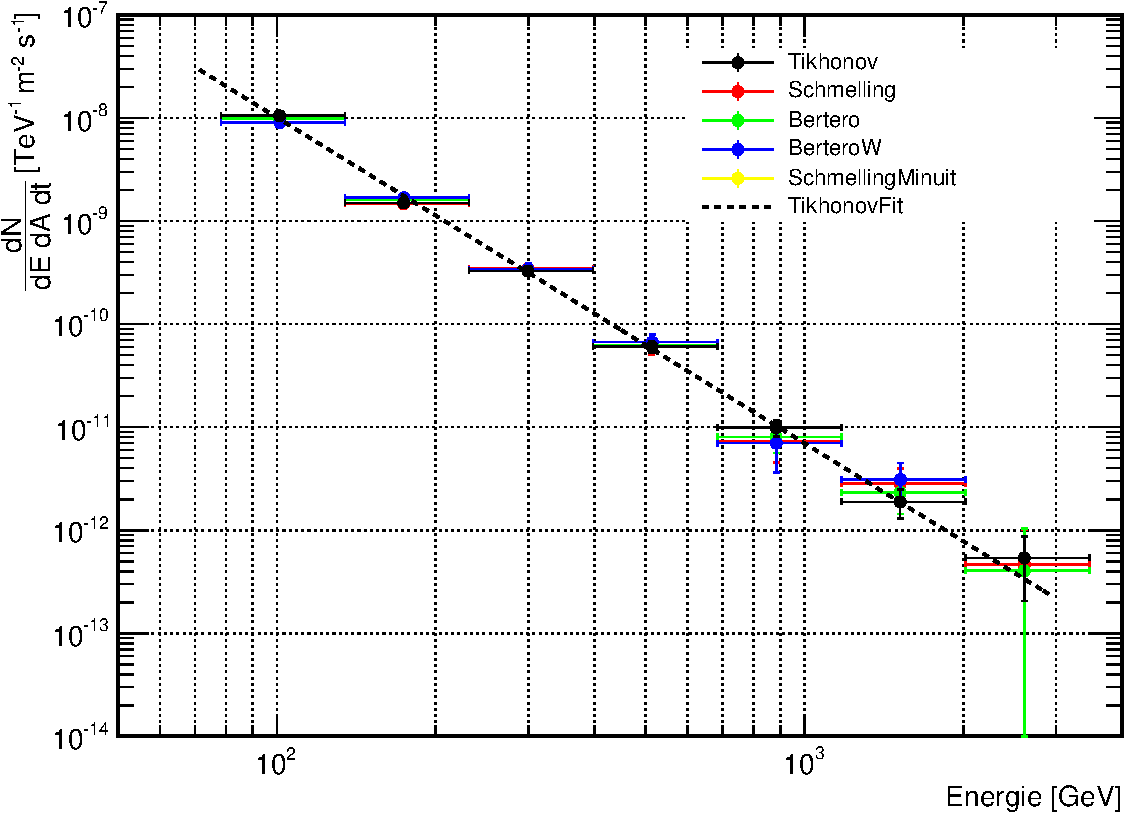
\includegraphics[width=0.8\textwidth]{./Plots/04_MrkAnalyse/Datenset4/Datenset4_Spektrum_Mrk421.pdf}
    \caption{Spektrum Mrk 421.}
    \label{Datenset4_Spektrum_Mrk421}
\end{figure}

Der Fit des entfalteten Spektrums mit Tikhonov-Regularisierung liefert folgendes Ergebnis:

\begin{equation}
 \frac{dF}{dE}=3,14 \cdot 10^{-10}\left( \frac{E}{0,3 \si{TeV}} \right)^{-3.16} \si{TeV^{-1}\,s^{-1}\,cm^{-2}}.
\end{equation}


\FloatBarrier

\subsection{Datenset 3}
\label{subsec:Datenset_3}

\subsubsection{Datencheck}
Der Datencheck für die Mono-Daten geschieht analog zum Datencheck der anderen Datensets.
Die Analyse beruht auf Daten auf Star-Level und nicht Superstar-Level wie vorher.
Tabelle \ref{tab:Datenset3-Mrk421} und Tabelle \ref{tab:Datenset3} zeigen, welche Mrk 421-und Off-Daten nach dem Datencheck übrig sind.
Ein Beobachtung von Crab gab es zu diesem Zeitraum nicht.

\begin{table}[!h]
\centering
\caption{Diese Tabelle zeigt, für welche Tage Mrk 421-Daten nach dem Datencheck zur Analyse zur Verfügung stehen.}
\label{tab:Datenset3-Mrk421}
\begin{tabular}{ll}
  \toprule
  Monat & Tage\\
  \midrule
  \midrule
Mai & 23., 25., 26., 27.\\
Juni & 15,. 19. \\
  \bottomrule
\end{tabular}
\end{table}


\begin{table}[!h]
\centering
\caption{Daten nach Datencheck}
\label{tab:Datenset3}
\begin{tabular}{lc}
  \toprule
  Quelle & Observationszeit\\
  \midrule
  \midrule
  Mrk 421 & 333min\\
  \midrule
  1ES1959 & 360min \\
  AE-Aqr & 54min  \\
  HD215227 & 649min \\
  M87 & 64min \\
  \bottomrule
  \bottomrule
\end{tabular}
\end{table}

\subsubsection{Energieschätzung}
Im Vergleich zu der Stereo-Analyse müssen für die Mono-Analyse ältere Programme benutzt werden.
Die RFs für die Disp-Bestimmung und Gamma-Hadron-Separation werden mit Hilfe von \textit{Osteria} erstellt.
Im Gegensatz zur Standardanalyse werden keine Look-Up-Tables zur Energieschätzung benutzt, sondern ebenfalls ein RF.

\subsubsection{Lichtkurve}
Nachdem die Ereignisse klassifiziert worden sind und ihnen ein Disp-Wert sowie eine geschätzte Energie zugeordnet worden sind, wird wieder eine Lichtkurve erstellt.
Dies geschieht mit Hilfe des Programms \textit{Fluxlc}.
Obwohl keine Crab-Daten zur Verfügung standen, um die Einstellungen für die Lichtkurve mit einem bekannten Fluss zu überprüfen, wird eine Lichtkurve für Mrk 421 erstellt.
Abb.\ref{Datenset3_LC_Mrk421} zeigt die Lichtkurve für Mrk 421.

\begin{figure}
    \centering
    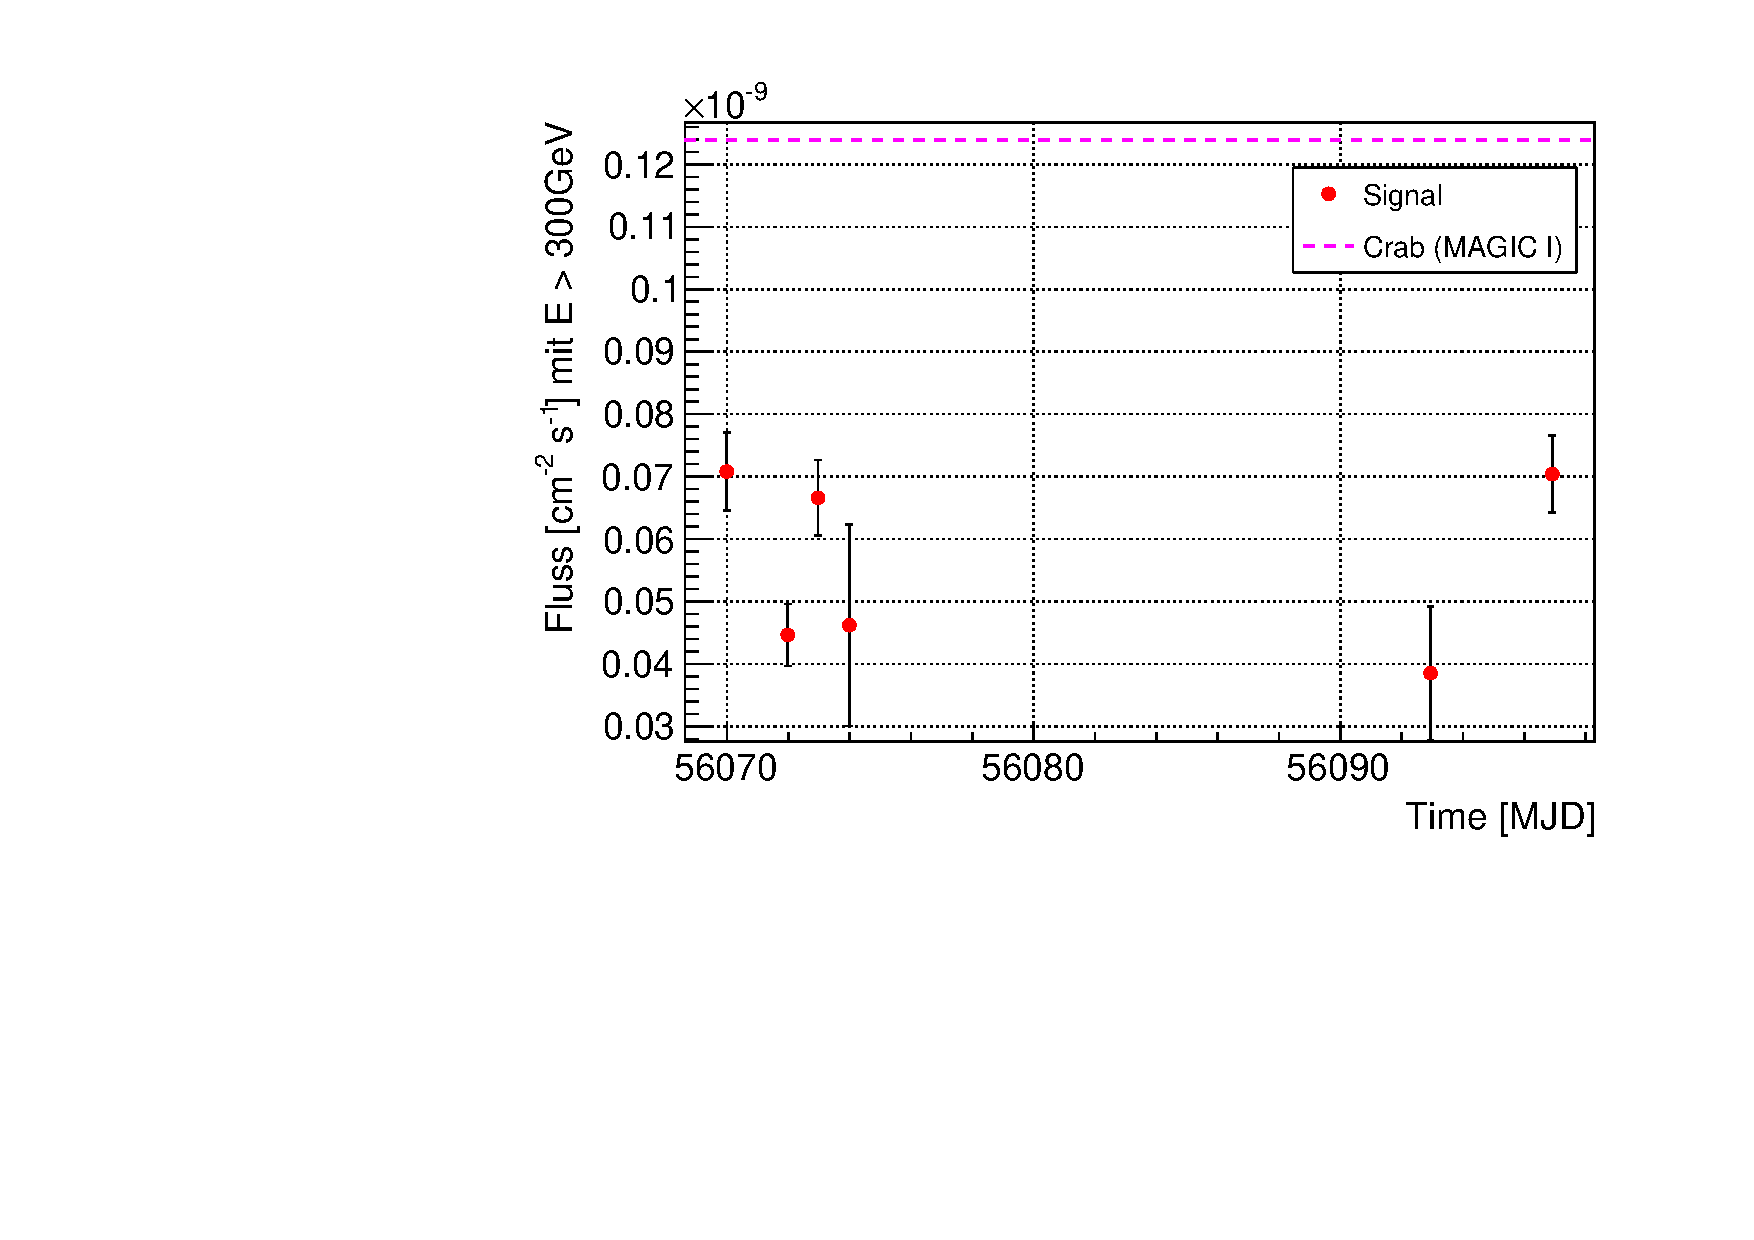
\includegraphics[width=0.8\textwidth]{./Plots/04_MrkAnalyse/Datenset3/Datenset3_Mrk421_LC.pdf}
    \caption{LC Mrk 421.}
    \label{Datenset3_LC_Mrk421}
\end{figure}

Es zeigt sich, dass der Fluss von Mrk 421 in diesem Zeitbereich genau wie in den anderen Zeitbereichen ebenfalls sehr niedrig ist.


\subsubsection{Spektrum}

Wie in Abb.\ref{Datenset3_Spektrum_Mrk421} zu sehen ist, werden die Daten abschließend wieder entfaltet.

\begin{figure}
    \centering
    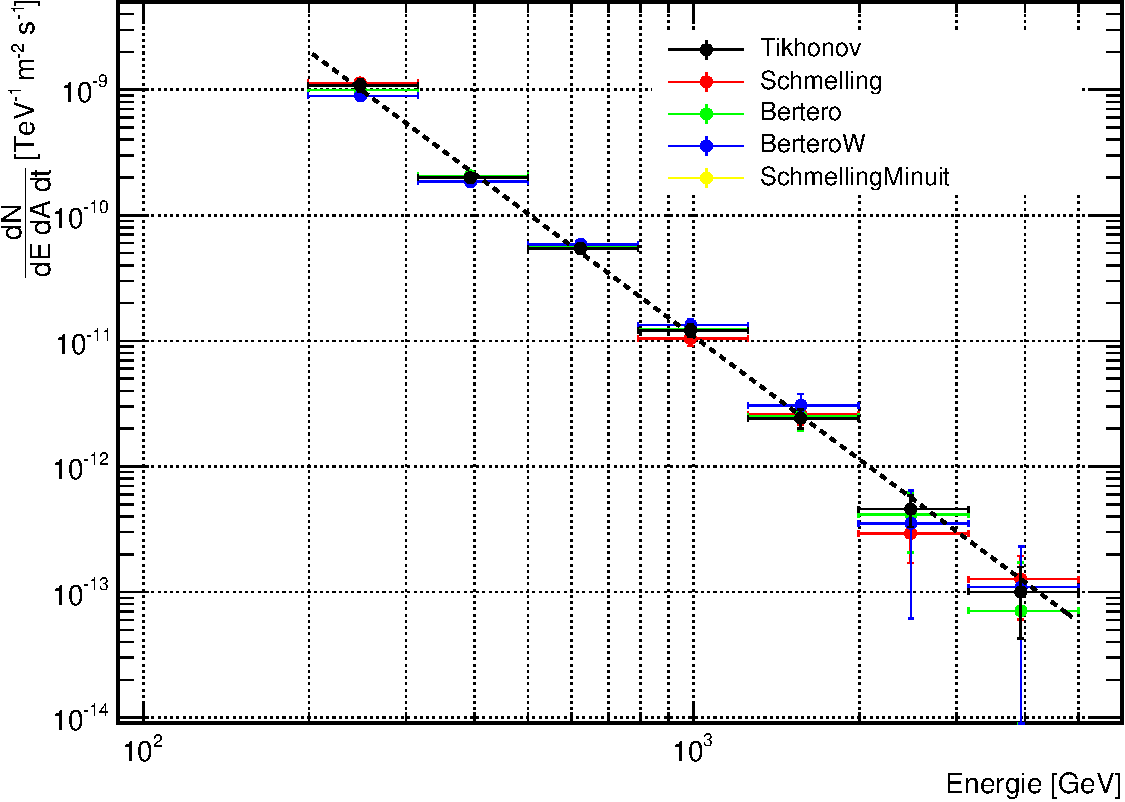
\includegraphics[width=0.8\textwidth]{./Plots/04_MrkAnalyse/Datenset3/Datenset3_Mrk421_Spektrum.pdf}
    \caption{Spektrum Mrk 421.}
    \label{Datenset3_Spektrum_Mrk421}
\end{figure}

Der Fit an die Datenpunkte liefert folgendes Ergebnis:

\begin{equation}
 \frac{dF}{dE}=(5,42 \pm 0.23) \cdot 10^{-10}\left( \frac{E}{\SI{0,3}{TeV}} \right)^{(-3.25 \pm 0.09)} \si{TeV^{-1}\,s^{-1}\,cm^{-2}}.
\end{equation}

\FloatBarrier


\section{Zusammenfassende Ergebnisse und Vergleich der Datensets}
\label{LC_Alles}

Nachdem für jedes Datenset einzelne Lichtkurven erstellt worden sind, sieht man in Abb.\ref{Alles_LC_Mrk421} nun alle Daten in einer Lichtkurve dargestellt.
Da zwischen dem 20.06.2012 und dem 10.12.2012 keine Daten von Mrk 421 genommen wurden, weil die MAGIC-I-Kamera außer Betrieb war und das Upgrade durchgeführt wurde, befindet sich eine große Lücke in der Lichtkurve.

\begin{figure}
    \centering
    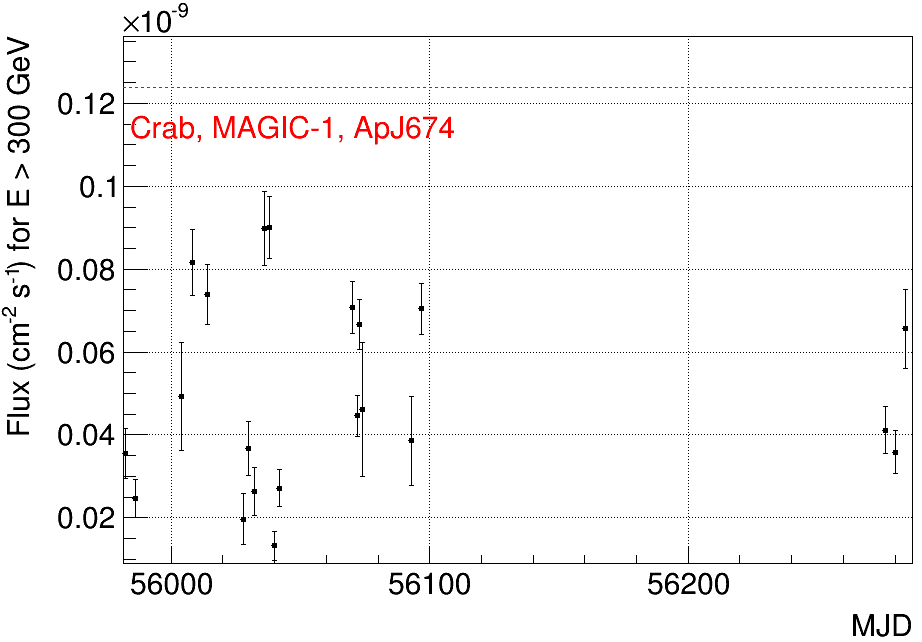
\includegraphics[width=0.8\textwidth]{./Plots/04_MrkAnalyse/Alles_LC.png}
    \caption{LC Mrk 421.}
    \label{Alles_LC_Mrk421}
\end{figure}

Es ist zu sehen, dass alle Datenpunkte etwa auf dem gleichen niedrigen Niveau liegen.
Der Fluss von Crab wird zu keinem Zeitpunkt erreicht. 
Physikalisch interessante Phänomene wie Flares sind auch nicht zu sehen.
%Im April 2013 trat beispielsweise ein Flare auf.
Verglichen mit dem gesamten Fluss von MAGIC zwischen Dezember 2004 und Dezember 2009 in \cite{DissBackes} ist der Fluss 2012 auf einem niedrigen Niveau.
Im Dezember 2006 war er an vielen Tagen genauso niedrig.

Im Gegensatz zu den Flares 2007 und 2008, bei denen der Fluss bis zu 20 mal so hoch war wie zu ruhigen Zeiten \cite{DissBackes}, ist der Fluss 2012 konstant niedrig.

Ein Vergleich mit dem Fluss zwischen Januar und Mai 2009 \cite{DissDiego} liefert ebenfalls das Ergebnis, dass sich sich Mrk 421 in einem ruhigen Zustand befindet.

In Tabelle \ref{tab:SpektraleIndizes} befinden sich die spektralen Indizes der Entfaltung der einzelnen Datensets.
Es ist zu sehen, dass die Indizes nahe beisammen liegen, abgesehen vom zweiten Datenset.
Da der spektrale Index eher hoch ist, ist der Fluss an hochenergetischen Teilchen gering

\begin{table}[!h]
\centering
\caption{Diese Tabelle zeigt die spektralen Indizes mit Fehler der einzelnen Datensets.}
\label{tab:SpektraleIndizes}
\begin{tabular}{lll}
  \toprule
  Datenset & Normierung $\left[\si{TeV^{-1}\,cm^{-2}\,s^{-1}}\right]$ & spektraler Index\\
  \midrule
  \midrule
Datenset 1 & $(1,42\pm 0,11)\cdot 10^{-10}$ & -3,01 $\pm$ 0,14 \\
Datenset 2 & $(2,74\pm 0,06)\cdot 10^{-10}$ & -2,64 $\pm$ 0,03 \\
Datenset 3 & $(5,42\pm 0,23)\cdot 10^{-10}$ & -3,25 $\pm$ 0,09 \\
Datenset 4 & $(3,14\pm 0,15)\cdot 10^{-10}$ & -3,16 $\pm$ 0,07 \\
  \bottomrule
\end{tabular}
\end{table}

